\documentclass[a4paper,12pt]{article}
\usepackage[a4paper,top=3cm,bottom=2cm,left=3cm,right=3cm,marginparwidth=1.75cm]{geometry}
\usepackage[brazil]{babel}
\usepackage[T1]{fontenc}
\usepackage[utf8]{inputenc}
\usepackage{amsmath}
\usepackage{MnSymbol}
\usepackage{wasysym}
\usepackage{hyperref}
\usepackage{color}
\definecolor{Blue}{rgb}{0,0,0.9}
\definecolor{Red}{rgb}{0.9,0,0}
\usepackage{esvect}
\usepackage{graphicx}
\usepackage{float}
\usepackage{indentfirst}
\usepackage{caption}
\usepackage{blkarray}
\newcommand\Mark[1]{\textsuperscript#1}
\usepackage{pgfplots}
\usepackage{amsfonts}
\usepackage[english, ruled, linesnumbered]{algorithm2e}
\usepackage{algorithmic}

\title{DMDGP: Um Problema Real}
\author{Guilherme Philippi\Mark{*}, orientado por Felipe Delfini Caetano Fidalgo\Mark{\dagger}\\Campus Blumenau\\Universidade Federal de Santa Catarina\\UFSC
\\guilherme.philippi@grad.ufsc.br\Mark{*}, felipe.fidalgo@ufsc.br\Mark{\dagger}}
\begin{document}
	\begin{titlepage}
		\newcommand{\HRule}{\rule{\linewidth}{0.5mm}} % Defines a new command for the horizontal lines, change thickness here
		\center % Center everything on the page
		%----------------------------------------------------------------------------------------
		%	HEADING SECTIONS
		%----------------------------------------------------------------------------------------
		\begin{center}
			
\includegraphics[scale=0.22]{logoufsc.jpg}
		\end{center}
		\vspace{1cm}
		
		\textsc{\LARGE \hspace{-0.17cm}Universidade Federal de Santa Catarina}\\[0.5cm] % Name of your university/college
		{\Large Centro de Blumenau \\ Departamento de Matemática}\\[1.5cm] % Major heading such as course name
		\textsc{\Large PIBIC \\ Relatório Final \vspace{1.5cm} }\\[2.0cm] % Minor heading such as course title
		
		%\textsc{\LARGE Universidade Federal de Santa Catarina}\\[0.5cm] % Name of your university/college
		%{\Large Centro de Blumenau \\ Departamento de Matemática}\\[1.5cm] % Major heading such as course name
		%\textsc{\Large PIBIC \\ Programa Institucional de Bolsas de Iniciação Científica \vspace{1.5cm} \\ {\bf PROJETO DE PESQUISA}}\\[2.0cm] % Minor heading such as course title
		
		%----------------------------------------------------------------------------------------
		%	TITLE SECTION
		%----------------------------------------------------------------------------------------
		
		\HRule \\[0.4cm]
		{ \LARGE \bfseries DMDGP: Um Problema Real} \\ [0.4cm] % Title of your document
		\HRule \\[2.5cm]
		
		%----------------------------------------------------------------------------------------
		%	AUTHOR SECTION
		%----------------------------------------------------------------------------------------
		
		\begin{minipage}{1\textwidth}
			\begin{center} \large
				Guilherme Philippi, orientado por Felipe Delfini Caetano Fidalgo
				\\g.philippi@grad.ufsc.br, felipe.fidalgo@ufsc.br 
			\end{center}
		\end{minipage} \\[2cm]
		
		
		{\large \today} % Date, change the \today to a set date if you want to be precise
		
		
		\vfill % Fill the rest of the page with whitespace
		
	\end{titlepage}
	
	
	\newpage
	\tableofcontents
	\newpage
	
	\begin{center}
		\large
		\textbf{Abstract}
	\end{center}
	
	This is a old abstract, dont read. In this paper, two subjects were presented in a disjointed form: The algebra of
	the quaternions and the Problem of Geometry of Molecular Distances. For the first,
	it begins with a historical introduction to quantum algebra and presents some of its	most basic results, monid of its partial or complete demonstrations, as it was found necessary. The same structure forms the second subject, but, due to its nature, a more literary and less formal approach was used. Starting from a contextualisation of the PGDM, some important tools were presented to model it, where, in possession of everything until then, the problem in question can be presented and a brief introduction to the study of its solution.
 
	
	\textbf{Keywords:} Quaternions, MDGP, Distance geometry, Optimization.
	 
	
	\vspace{2cm}	
	\begin{center}
		\large
		\textbf{Resumo}
	\end{center}

	Este é um resumo velho, nem leia. Neste documento foram apresentados dois assuntos de forma disjunta: A álgebra dos quatérnios e o Problema de Geometria de Distâncias Moleculares. Para o primeiro, inicia-se com uma introdução histórica à álgebra de quatérnios e apresenta-se alguns de seus resultados mais básicos, monidos de suas demonstrações parciais ou completas, conforme achou-se necessário. A mesma estruturação forma o segundo assunto, porém, devido a sua natureza, utilizou-se uma abordagem mais literária e menos formal. Partindo de uma contextualização do PGDM, apresentou-se algumas ferramentas importantes para modelá-lo, onde, de posse de tudo até então, pode-se apresentar de fato o problema em questão e uma brevê introdução ao estudo de sua solução. 
	
	\textbf{Palavras-chave:} Quatérnios, PGDM, Geometria de Distâncias, Otimização.
	
	
	\newpage
	\section{Introdução}
	Existe uma relação muito forte com a forma geométrica das moléculas orgânicas e suas funções em organismos vivos. Pode-se fazer uma analogia destes organismos com um grande quebra-cabeça, cheio de peças tão variadas quanto se queira, onde cada peça tem um local específico no grande quebra-cabeça, de forma que sua posição e função é dado justamente pela forma geométrica de cada peça. Imagine este grande quebra-cabeça de forma tridimensional ao invés de plana, com peças em formatos diversos e escalafobéticos, logo, você não estará tão longe de entender como funciona um organismo vivo.
	
	Outrora, em pesquisas sobre a molécula de DNA (ácido desoxirribonucleico), descobriu-se que essa era parte fundamental da produção de um dos pilares para a vida: a proteína. Esta será o alvo principal deste estudo e possuí uma gama extensa de funções em nosso organismo --- como se fossem as tais peças do quebra-cabeça da analogia acima. Podemos dizer que somos feitos de proteínas. Organismos vivos lutam constantemente contra a desorganização intrínseca do universo e as proteínas tem papel importantíssimo nessa luta. São elas as estruturas que utilizamos para nos organizar, gerando informação, ao possibilitarem um mecanismo procedural natural para a vida, como com o seu papel no transporte de oxigênio (hemoglobina), na proteção do corpo contra organismos patogênicos (imunoglobulina), com a catalização de reações químicas (apoenzima), além de outras inúmeras funções primordiais no nosso organismo \cite{fidalgotese}. Perceba a importância fundamental em estudar a estrutura geométrica de cada uma dessas proteínas e sua relação com suas funções.
	
	Por conta dessa motivação tem-se esforços como o de Kurt Wüthrich, que propôs que se utilizasse experimentos de \textit{Ressonância Magnética Nuclear}
	(RMN) para calcular a estrutura tridimensional de uma molécula de proteína, ganhando o premio Nobel da Química em 2002 \cite{RMNproteinWrutrich}. Porém, a partir dessa estratégia tivemos novos problemas. A RMN não tem como resultado a estrutura tridimensional de uma proteína, mas sim distâncias entre átomos relativamente próximos que compõem a proteína. Para poder calcular a estrutura de uma proteína a partir dessas distâncias, surgira um novo problema, conhecido na literatura como \textit{Problema de Geometria de Distâncias Moleculares}, ou simplesmente, MDGP \cite{carlileGDandAplications}.
	
	Ao longo desse texto estudaremos este problema, suas variações, seus problemas relacionados, as ferramentas que nos facilitarão a resolve-los, suas soluções e as complexidades relacionadas a estas soluções.
	
	\newpage

	\section{Materiais e Métodos}
	
	\newpage
	
	\section{Grafos: Aspectos Gerais}
	
	\newpage
	
	\section{Um Passeio pela Bioquímica}
	A bioquímica é a ciência que busca explicar as formas e funções biológicas em termos químicos, uma tarefa muito divertida, porém, complicada. Já no século XVIII, os químicos percebiam a grande diferença entre o mundo inanimado e o mundo vivo: Antoine-Laurent Lavoisier (1743-1794) constatou a relativa simplicidade do ``mundo mineral'' --- não orgânico --- comparada a complexidade dos ``mundos animal e vegetal'' \cite{bioquimicaLehninger}. Ele sabia que esses últimos eram constituídos de moléculas ricas nos elementos carbono, oxigênio, nitrogênio e fósforo, que, devido sua abundância na natureza somada com as suas características químicas, são ótimos para constituírem a complexidade da vida.

	\subsection{Carbono}
	A química dos organismos vivos está organizada em torno do carbono, pois este é muito comum na natureza e possuí uma ótima propriedade estrutural: O carbono pode formar ligações simples estáveis com até quatro outros átomos. De fato, o carbono constitui mais da metade do peso seco das células. 
	
	Sabe-se, através de experimentos de cristalografia \cite{ramachandran1974MolStructure}, muito sobre a geometria das ligações dos átomos de uma proteína. Em particular, as quatro ligações simples do carbono formam um tetraedro (vide Figura ~\ref{fig:carbono}, retirada de \cite{bioquimicaLehninger}) com ângulos de 109,5\textdegree entre duas ligações quaisquer e comprimento médio de ligação de 1,54\AA\footnote[1]{Unidade física para distâncias atômicas é o Ângstron (\AA), onde equivale a 1\AA = $10^{-10}$ m.}. Existe também uma outra característica muito importante para nós nas ligações do carbono: Sabe-se que as ligações simples podem rotacionar livremente (a menos que grupos muito grandes ou altamente carregados estejam ligados aos átomos de carbono, onde, neste caso --- e, na verdade, esse é o caso comum ---, a rotação é regida pelo equilíbrio de forças na molécula \cite{carlileTese}, que pode ser limitada), enquanto que as ligações duplas são mais curtas (em torno de 1,34\AA) e não permitem rotação. Perceba também o plano formado pelos átomos A, B, X e Y na Figura ~\ref{fig:carbono}.

	\begin{figure}[H]
		\begin{center}
			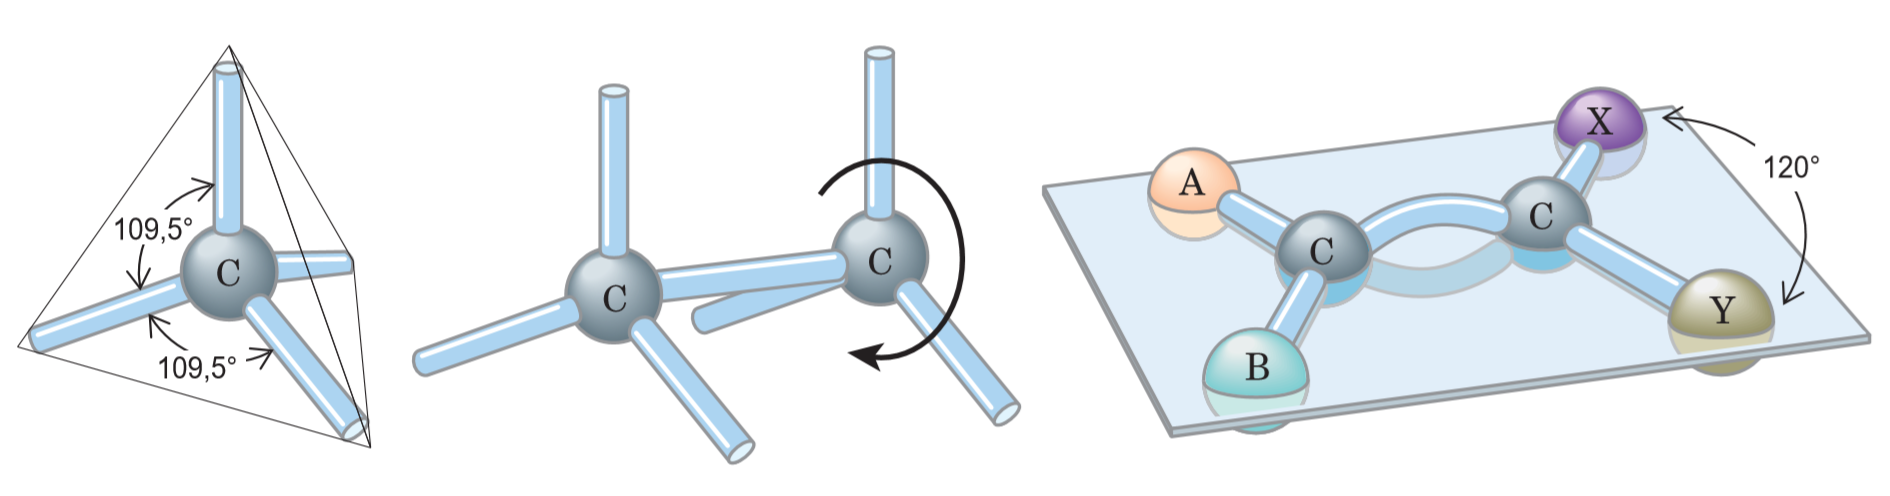
\includegraphics[width=1\linewidth]{carbono.png}
		\end{center}
		\caption{Geometria da ligação do carbono.}
		\label{fig:carbono}
	\end{figure}

	A versatilidade das ligações covalentes do carbono podem formar cadeias lineares, ramificadas e estruturas cíclicas. Nenhum outro elemento químico consegue formar moléculas com tanta diversidade de tamanhos, formas e composição.
	
	\subsection{Classificação Macromolecular}
	As células contém um conjunto universal de moléculas pequenas. Mas como podemos discutir sobre o que é uma molécula pequena? Devemos definir uma forma de comparar os tamanhos moleculares. Na literatura existem duas medidas principais para esse fim, com uma relação bem definida entre si, tratam-se do \textit{peso molecular} (ou \textit{massa molecular relativa}), denominado $M_r$ e da \textit{massa molecular}, denotada simplesmente por $m$.
	
	O peso molecular é definido como uma relação direta da massa da molécula da substância estudada com um duodécimo da massa do carbono-12 ($^{12}C$, em torno de $1,9926\times 10^{-23}$ gramas), note que, como $M_r$ é uma razão, não possui dimensão associada. Já a massa molecular é apenas a massa da molécula (ou massa molar) sobre o número de Avogadro --- que é definida como sendo o número de átomos por mol de uma determinada substância. Esta, diferente da massa molecular relativa, possui dimensão e é expressa em dáltons (abreviado Da) e um dálton equivale a um duodécimo da massa do carbono-12 --- donde deduze-se facilmente a relação entre massa molecular e peso molecular.
	
	Os organismos vivos são constituídos por moléculas de características muito diversas. Existe uma coleção de aproximadamente mil moléculas consideradas pequenas ($M_r$ ${\sim}100$ a ${\sim}500$) diferentes dissolvidas na fase aquosa das células \cite{bioquimicaLehninger}. Nessa coleção está contido os aminoácidos comuns, nucleotídeos, açúcares e seus derivados fosforilados e ácidos mono, di e tricarboxílicos. Porém, neste estudo, estaremos mais preocupados com moléculas significativamente maiores, chamadas \textit{macromoléculas}.
	\subsubsection*{Macromoléculas}
	As macromoléculas são as principais constituintes das células. São polímeros\footnote[1]{Polímeros são moléculas formadas a partir de repetições de unidades estruturais menores, chamadas \textit{meros} ou \textit{monômeros}. Daí o nome, poli-meros $\approx$ vários-meros.} com peso molecular acima de ${\sim}5.000$. Polímeros menores são chamados de \textit{oligômeros} --- do grego, ``oligos'' significa ``pouco''. Proteínas (principal molécula do nosso estudo), ácidos nucleicos (DNA, RNA) e polissacarídeos são macromoléculas feitas de monômeros cujos pesos moleculares são de 500 ou menos, porém, como apresentam um grande número dessas subunidades, possuem um alto peso molecular --- até 1 milhão para proteínas e até vários bilhões para ácidos nucleicos. A síntese de macromoléculas é a atividade mais custosa energeticamente das células.
	
	Tanto as proteínas quanto os ácidos nucleicos são polímeros lineares (isto é, que não possuem ramos ligados as suas cadeias principais, agindo como um longo fio contínuo) feitos de subunidades monoméricas bem mais simples, donde esta sequência específica de meros é que dá as informações sobre a sua estrutura tridimensional e suas funções biológicas associadas \cite{bioquimicaLehninger}.
	
	Em especial, as proteínas são constituídas por um conjunto de monômeros muito bem conhecidos e catalogados, chamados \textit{aminoácidos}. As proteínas constituem a segunda maior fração da célula, só perdendo para a água. Provavelmente são as mais versáteis de todas as biomoléculas: Algumas tem atividade catalítica e funcionam como enzimas, outras servem como elementos estruturais, receptoras de sinais, ou transportadoras que carregam substâncias específicas para dentro ou fora das células.  
	
	\subsection{Configuração Molecular}
	No mundo biomolecular, toda a informação sobre uma molécula é dada pela sua estrutura (também chamada de \textit{estereoquímica}), logo, suas ligações covalentes e seus grupos funcionais (subestruturas padrões associadas) são trivialmente importantes para definir seu bom funcionamento. Devido a característica rotacional das ligações simples do carbono, existem muitas moléculas (chamadas \textit{estereoisômeros}) com a mesma fórmula molecular e ligações químicas, mas com diferentes configurações espaciais, o que pode mudar completamente suas funções. 
	
	De maneira simples, podemos identificar estereoisômeros pelo fato de que eles possuem as mesmas propriedades químicas, porém, não podem ser convertidos entre si sem que haja a quebra de uma ou mais ligações covalentes. Isto se dá pela presença de ligações duplas (devido a limitação na sua rotação) ou pela presença de \textit{centros quirais}, onde a molécula rotacionada não pode corresponder a sua imagem especular (conforme Figura ~\ref{fig:quiral}, extraída de \cite{bioquimicaLehninger}). Um átomo de carbono com quatro ligações diferentes é considerado assimétrico e é chamado de centro quiral --- do grego, \textit{chiros} quer dizer "mão", parafraseando estas estruturas com a relação da mão direita com a esquerda. Logo, se existir um centro quiral, sempre haverá pelo menos duas possibilidades para configuração.
	 
	\begin{figure}[H]
		\begin{center}
			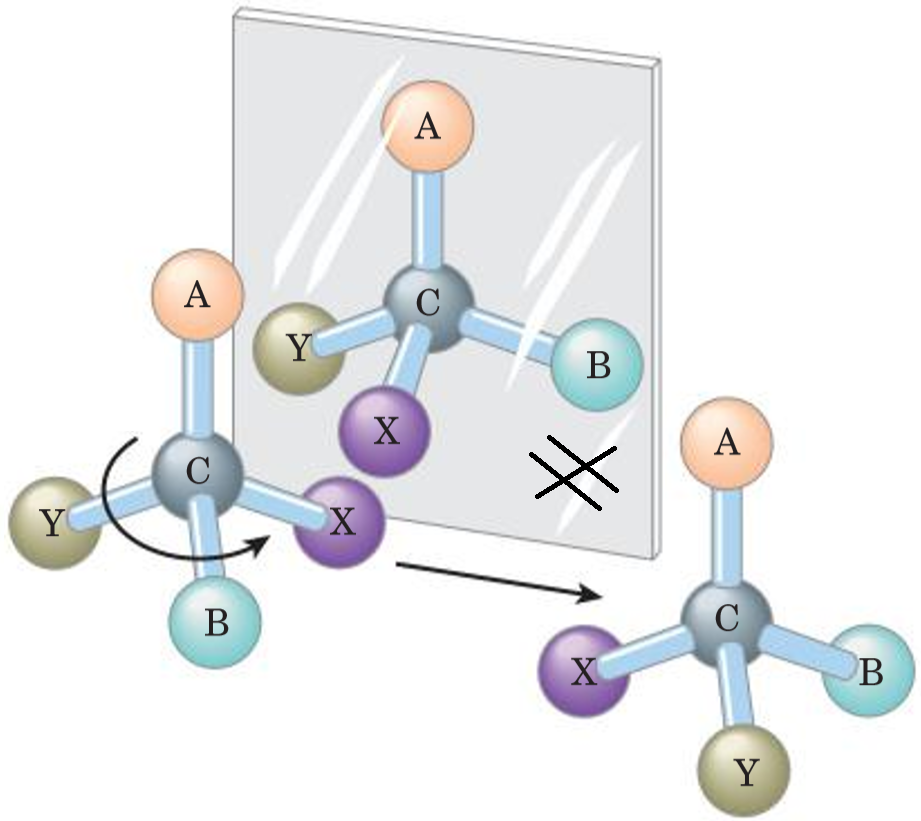
\includegraphics[width=0.45\linewidth]{quiral.png}
		\end{center}
		\caption{Ilustração de uma molécula quiral.}
		\label{fig:quiral}
	\end{figure} 
	
	 Outro conceito que nos será importante no futuro, a \textit{conformação molecular} é a disposição dos átomos no espaço que pode ser mudada por rotação em torno de ligações simples, sem quebrar ligações covalentes. Estes ângulos possíveis tem posições mais estáveis e instáveis do ponto de vista energético, conforme mostra o gráfico da Figura ~\ref{fig:carener}. Podemos tentar descobrir a conformação mais provável de uma molécula minimizando a somatória de todas as forças atuantes na molécula \cite{carlileTese}. 
	
	\begin{figure}[H]
		\begin{center}
			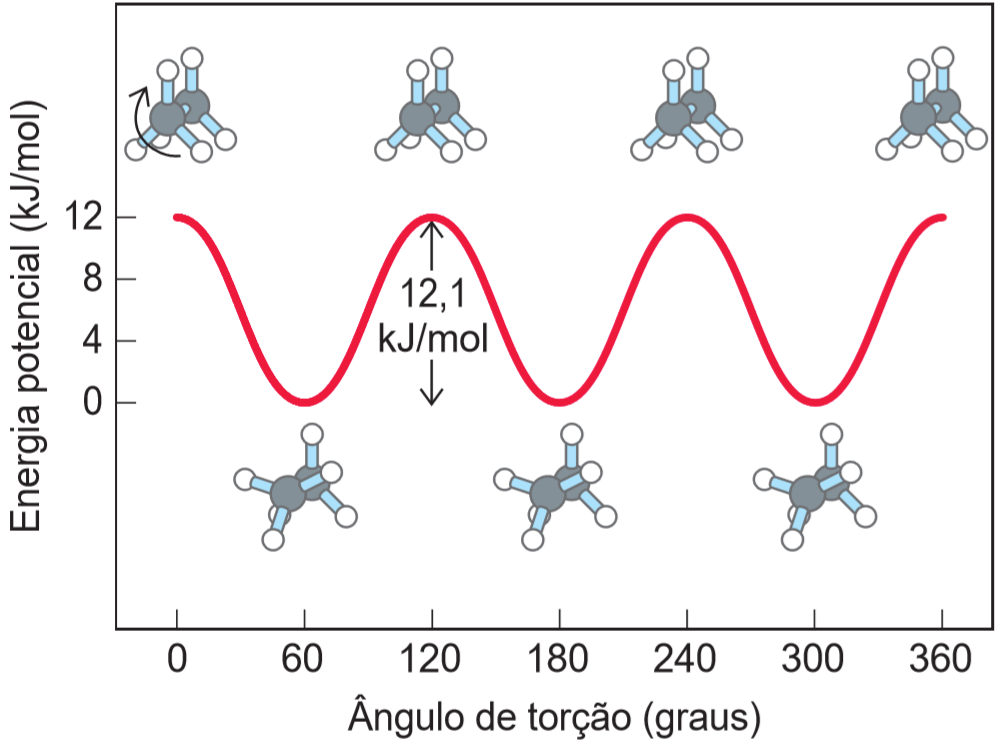
\includegraphics[width=0.55\linewidth]{carbonoenergia.png}
		\end{center}
		\caption{Conformações e Equilíbrio de Energia \cite{bioquimicaLehninger}.}
		\label{fig:carener}
	\end{figure} 
	
	Para compreender melhor como serão as configurações das moléculas que trataremos nesse texto (proteínas), vale nos preocuparmos com as subestruturas do qual eles são formados. 
	
	\subsection{Aminoácidos}
	As proteínas são longas cadeias lineares de aminoácidos ligados por um tipo específico de ligação (chamada \textit{peptídica}), a qual é característica por ter como resíduo uma molécula de água. São vinte tipos diferentes de aminoácidos encontrados normalmente na natureza, sendo esses muito bem conhecidos e catalogados. O primeiro a ser descoberto foi a asparagina, em 1806; o ultimo foi a treonina, descoberto em 1938 \cite{bioquimicaLehninger}. Vale mencionar que, além destes vinte aminoácidos mais comuns, há vários outros menos frequentes, porém não constituem as proteínas.
	
	Destes vinte aminoácidos comuns (disponíveis no Apêndice C), dezenove compartilham da mesma estrutura principal \cite{fidalgotese} --- estes são chamados $\alpha$-aminoácidos. Eles tem um grupo carboxílico e um grupo amina ligados ao mesmo átomo de carbono (o carbono $\alpha$), além de mais um hidrogênio (chamado hidrogênio $\alpha$) e, em sua última ligação, uma cadeia R que é o que diferencia cada aminoácido. Essa estrutura é ilustrada na Figura ~\ref{fig:amino}. O único aminoácido que difere disso é a Prolina, que possui como cadeia R um anel aromático que se fecha no nitrogênio (que no padrão mencionado há um grupo amina).
	
	\begin{figure}[H]
		\begin{center}
			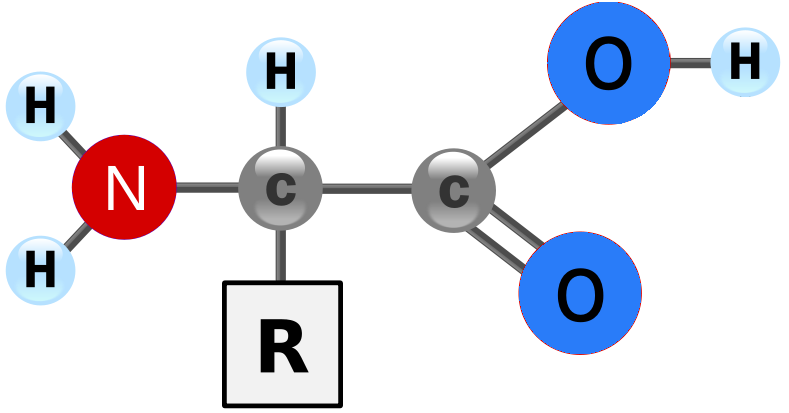
\includegraphics[width=0.35\linewidth]{amino.png}
		\end{center}
		\caption{Estrutura padrão de um $\alpha$-aminoácido.}
		\label{fig:amino}
	\end{figure}
	
	Por tanto, há uma noção prévia de qual tipo de estrutura esperar ao analisar uma molécula de proteína. Existe uma estrutura conhecida e repetitiva para os átomos.
	
	Para todos os aminoácidos comuns, exceto a glicina, o carbono $\alpha$ está ligado com quatro outros átomos diferentes entre si (na glicina temos R como apenas mais um hidrogênio, sendo o aminoácido mais simples), o que transforma o carbono $\alpha$ em um centro quiral. Logo, cada aminoácido (menos glicina) tem sempre dois estereoisômeros possíveis. Porém, na verdade, apenas um destes ocorrê naturalmente nas proteínas \cite{bioquimicaLehninger}.
	
	\subsubsection*{Ligação Peptídica}
	A ligação entre dois aminoácidos é feita de modo covalente por meio de desidratação do grupo $\alpha$-carboxílico de um com o grupo $\alpha$-amina do outro --- ou seja, ligar o carbono final de um no nitrogênio inicial do outro, liberando um oxigênio e dois hidrogênios, que formam uma molécula de água. Essa ligação, também chamada de resíduo (devido a liberação da água), forma um dipeptídeo. 
	
	Quando muitos aminoácidos se juntam, o produto é chamado de polipeptídeo. Perceba que os termos ``polipeptídeo'' e ``proteína'' parecem dirigir-se as mesmas moléculas, porém, a diferença está na massa molecular: As moléculas com massa abaixo de 10.000 são ditas polipeptídeos, enquanto as maiores que essas são consideradas proteínas. Os comprimentos dessas cadeias variam significativamente. O citocromo c humano tem apenas 104 aminoácidos, enquanto, no outro extremo, a titina (relacionada ao músculo de vertebrados) possui aproximadamente 27.000 aminoácidos e uma massa molecular de cerca de 3.000.000. No geral, as proteínas naturais contém menos de 2.000 aminoácidos \cite{bioquimicaLehninger}.
	
	Outra característica muito importante das ligações peptídicas é de que elas se comportam semelhantemente a ligações covalentes duplas dos carbonos. Estudos envolvendo difração de raios X em cristais de aminoácidos e polipeptídeos descobriram que a ligação peptídica $C-N$ é de alguma forma mais curta que a ligação de uma amina simples, e que os átomos associados a ligação peptídica estão todos co-planares (conforme Figura ~\ref{fig:peptidica}). Perceba que também são rígidos, não sendo possível a rotação. Essa é uma propriedade muito útil que também nos será importante, descoberta de 1930 que se deve a Linus Pauling e Robert Corey.
	
	\begin{figure}[H]
		\begin{center}
			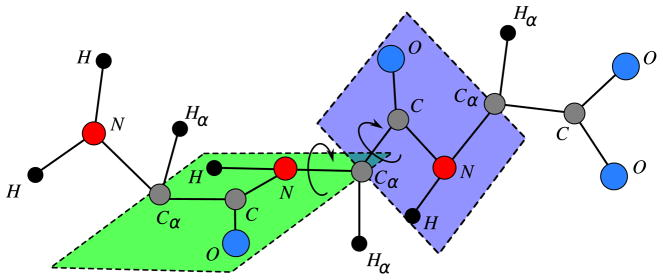
\includegraphics[width=0.8\linewidth]{peptide.jpg}
		\end{center}
		\caption{O grupo peptídico planar \cite{carlile:MinimalOrder}.}
		\label{fig:peptidica}
	\end{figure}

	\subsection{Estrutura das Proteínas}
	A estrutura de proteínas pode ser descrita em quatro níveis de importante hierarquia conceitual, conforme pode ser visto na Figura ~\ref{fig:protest}, retirado de \cite{bioquimicaLehninger}. A estrutura primaria consiste da mais detalhada, sendo de fato os polímeros de aminoácidos; Estes, por sua vez, formam alguns arranjos particularmente estáveis, que dão origem a padrões estruturais recorrentes, que chamamos de \textit{estruturas secundárias} (como as hélices $\alpha$, as duplas hélices etc..). A estrutura terciária descreve todos os aspectos do enovelamento tridimensional de um polipeptídeo, ou seja, define quais serão as forças atuantes na molécula --- que da origem a sua conformação estável, que minimiza a energia livre de Gibbs do sistema. Quando existem mais estruturas terciárias em uma proteína, chamamos a junção destas de estrutura quaternária.	
	
	\begin{figure}[H]
		\begin{center}
			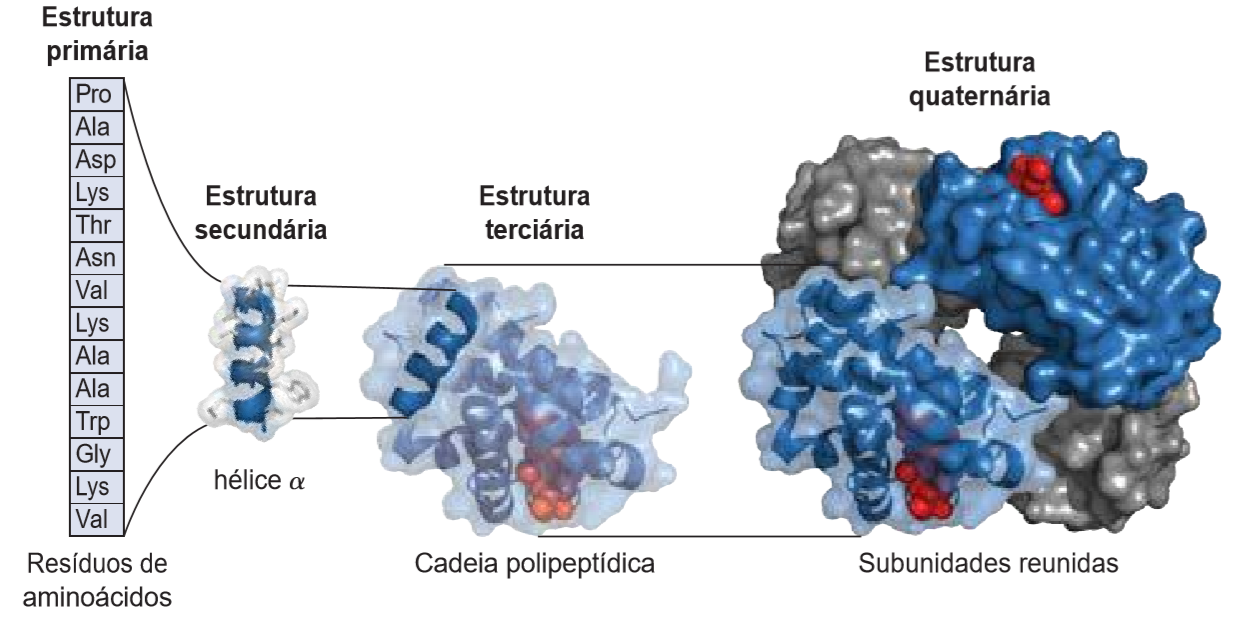
\includegraphics[width=1\linewidth]{protest.png}
		\end{center}
		\caption{Níveis de estrutura das proteínas exemplificados na Hemoglobina.}
		\label{fig:protest}
	\end{figure}
	
	Em especial, as diferentes configurações da estrutura primária --- que pode mudar drasticamente entre estruturas primárias diferentes na mesma molécula --- nos é mais informativa. A estrutura primária de uma proteína determina como ela se dobra em sua estrutura tridimensional, devido os ângulos e distâncias bem definidos de suas ligações entre átomos, que da a sua estrutura especial; o que, por sua vez, determina a função da proteína --- como no exemplo da Figura ~\ref{fig:protest}, onde a estrutura da hemoglobina é que permite que átomos de oxigênio ``encaixem'' nela, possibilitando o transporte desse átomo pelo organismo, que é sua função (e só o é dado sua estrutura tridimensional). 
	
	Por sua relação com a estrutura tridimensional e, logo, função das proteínas, vamos nos concentrar em estudar a subdivisão de estruturas primárias. 
	
	\subsubsection*{A Cadeia Principal de uma Proteína}
	Quando se estuda proteínas a nível dos aminoácidos, não tardamos a perceber que elas possuem uma estrutura repetida muito interessante do ponto de vista bioquímico. Trata-se da \textit{cadeia principal} de uma proteína, também chamada de \textit{Backbone} --- espinha dorsal, em tradução literal, fazendo alusão a importância desta estrutura. Perceba que os vinte aminoácidos que compõem as proteínas possuem sempre os mesmos três átomos ligados em sequência (Figura ~\ref{fig:backbone}): $N-C_\alpha-C$, através de ligações covalentes em torno do $C_\alpha$ e da ligação peptídica $C-N$ entre aminoácidos.
	
	\begin{figure}[H]
		\begin{center}
			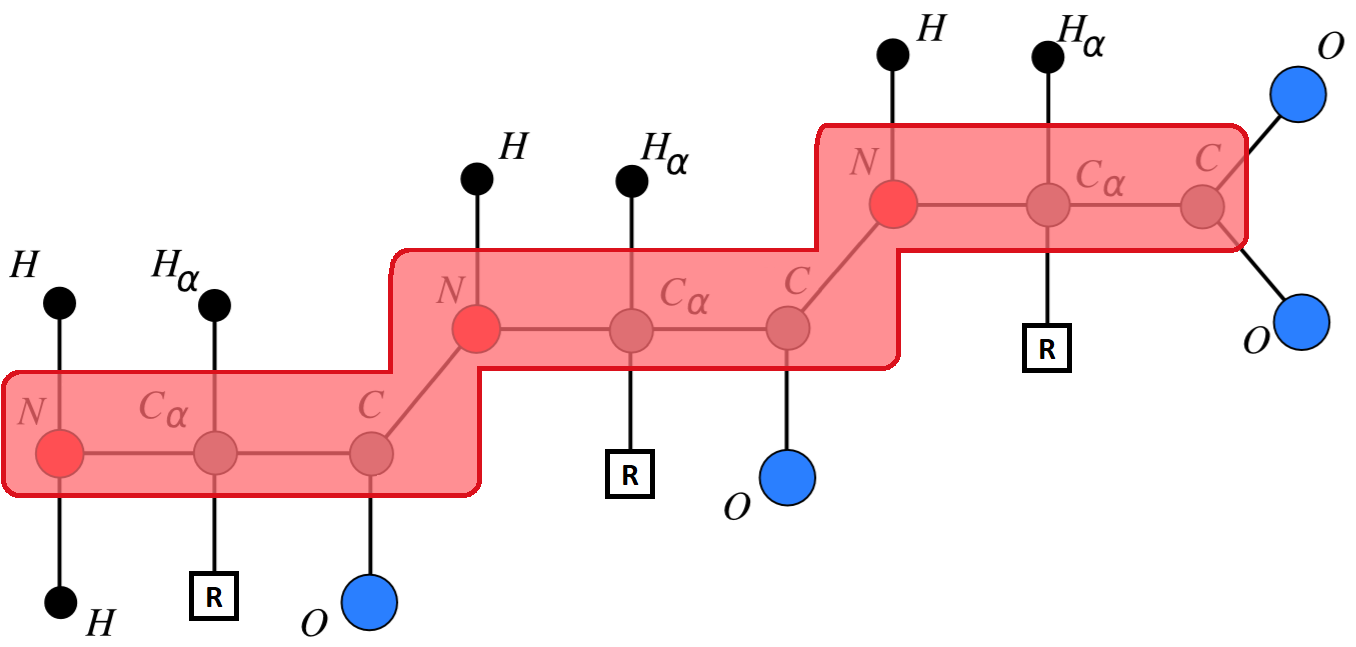
\includegraphics[width=0.8\linewidth]{backbone.png}
		\end{center}
		\caption{Representação da cadeia principal da proteína, adaptada de  \cite{carlile:MinimalOrder}}.
		\label{fig:backbone}
	\end{figure}
	
	Outra informação bastante útil sobre esta cadeia principal é que, devido dados experimentais de cristalografia, sabe-se sobre a geometria média dessa subestrutura \cite{ramachandran1974MolStructure}, onde os comprimentos e ângulos entre  as ligações dos átomos que a formam são fixas, na média, a menos de erros de medida. Vide Figura ~\ref{fig:rama}, extraída do texto original --- por razões emocionais --- de Ramachandran \textit{et al}, um dos precursores deste estudo.
	
	\begin{figure}[H]
		\begin{center}
			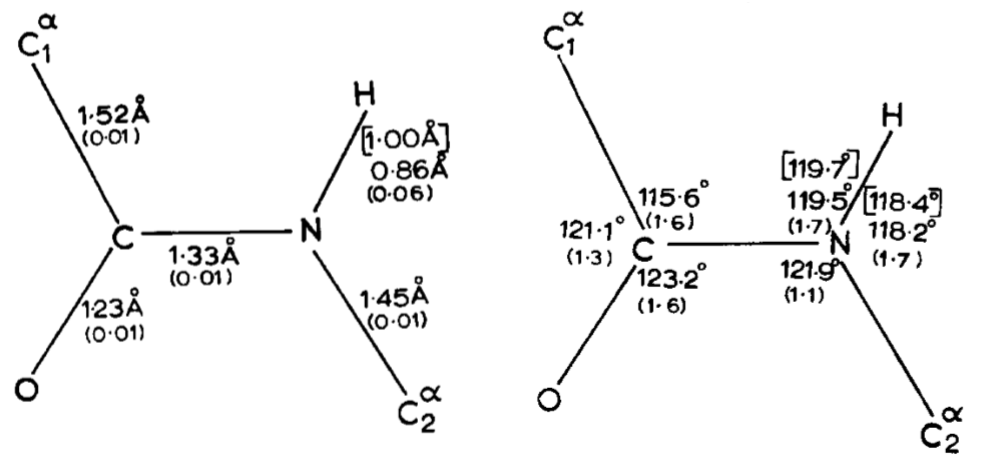
\includegraphics[width=0.8\linewidth]{rama.png}
		\end{center}
		\caption{Dados de ângulos e distâncias médios de ligações em um aminoácido.}
		\label{fig:rama}
	\end{figure}
	
	
	\subsection{\textit{Worldwide Protein Data Bank}}
	Já foi possível perceber a grande variedade de diferentes configurações possíveis para as proteínas. Com isso, há a necessidade de se estudar cada uma explicitamente, através de experimentos, catalogando e guardando essas informações. Esse grande esforço para entender o mundo das macromoléculas se deixa transparecer com o repositório \textit{Worldwide Protein Data Bank} --- ou simplesmente wwPDB \cite{wwPDB}.
	
	Este é um repositório online e público onde estão guardadas todas os dados de proteínas e ácidos nucleicos já catalogados, em especial dados de suas estruturas 3D (posições x, y e z de cada um dos átomos que a constituem). Auxiliando tanto pesquisadores, quanto professores e estudantes, popular essa base de dados é um grande esforço em conjunto de físicos, biólogos, bioquímicos e vários outros profissionais de diversas áreas do conhecimento de todo o mundo.
	
	\subsubsection*{Arquivo PDB}
	Quando se quer estudar uma proteína no repositório PDB, base fazer o \textit{download} do arquivo PDB da molécula (extensão ``.ent''). Esse é um arquivo de estruturas tridimensionais de macromoléculas biológicas determinadas experimentalmente, que descrevem as coordenadas espaciais de cada átomo cuja posição foi determinada (muitas das estruturas catalogadas não estão completas); também existem dados adicionais sobre informações de como as estruturas foram determinadas, os dados práticos dos experimentos, a precisão associada aos dados e tudo mais que quem estiver criando o documento achar necessário para aquela macromolécula.
	
	Tecnicamente, o arquivo PDB trata-se de uma representação estruturada dos dados moleculares e experimentais da proteína. Ele é separado por seções, onde cada seção pode possuir subseções. São elas: 
	\begin{itemize}
		\item \textbf{Seção Title} - Contem a descrição da molécula;
		\vspace{-0.3cm}
		
		\item \textbf{Seção Remark} - Vários comentários sobre anotações de entrada com mais profundidade que os registros padrões;
		\vspace{-0.3cm}
		
		\item \textbf{Seção Primary structure} - Sequências peptídicas ou nucleotídicas especificadas para serem posteriormente utilizadas, diminuindo a repetição do arquivo;
		
		\vspace{-0.3cm}
		\item \textbf{Seção Heterogen} - Descrição de grupos presentes não padronizados --- Visto que proteínas também podem conter materiais inorgânicos, como o ferro presente na hemoglobina (vide Figura ~\ref{fig:protest});
		\vspace{-0.3cm}
		
		\item \textbf{Seção Secondary structure} - Descrição das estruturas secundárias presentes na molécula;
		
		\vspace{-0.3cm}
		\item \textbf{Seção Connectivity annotation} - Descrição das conectividade químicas da molécula;
		\vspace{-0.3cm}
		
		\item \textbf{Seção Miscellaneous features} - Descrição dos recursos dentro da macromolécula;
		\vspace{-0.3cm}
		
		\item \textbf{Seção Crystallographic} - Descrição de parâmetros da cristalografia, quando o experimento utiliza esta metodologia;
		
		\vspace{-0.3cm}
		\item \textbf{Seção Coordinate transformation} - Matrizes como operadores de transformação das coordenadas;
		\vspace{-0.3cm}
		
		\item \textbf{Seção Coordinate} - Dados de coordenadas atômicas, a seção que mais vamos utilizar;
		\vspace{-0.3cm}
		
		\item \textbf{Seção Connectivity} - Citação das conexões químicas entre os átomos;
		\vspace{-0.3cm}
		
		\item \textbf{Seção Bookkeeping} - Resumo das características totais do arquivo e o marcador de fim de arquivo.
	\end{itemize}
	
	Como o arquivo é significativamente extenso, não entraremos em detalhes neste texto sobre as características detalhadas de cada uma das seções apresentadas. Porém, vale mencionar o tipo de entrada ATOM, presente na seção Coordinate, pois essa é a entrada que compõe a maior parte dos arquivos PDB, além de ser a de nosso interesse principal.
	
	A entrada ATOM tem como objetivo descrever detalhes de cada átomo específico da molécula. Ela segue um padrão indentado, onde cada dado é caracterizado pela sua posição na linha (coluna). Segue principais dados da entrada e suas respectivas colunas na Tabela ~\ref{table:atom}.
	
	\begin{table}[h!]
		\centering
		\begin{tabular}{ |c|c| } 
			\hline
			Código serial do átomo & 7-11 \\ 
			\hline
			Nome do átomo & 13-16 \\ 
			\hline
			Nome do resíduo que pertence & 18-20 \\ 
			\hline
			Identificador da cadeia & 22 \\ 
			\hline
			Código serial de dentro do resíduo & 23-26 \\ 
			\hline
			Coordenada x & 31-38 \\ 
			\hline
			Coordenada y & 39-46 \\ 
			\hline
			Coordenada z & 47-54 \\ 
			\hline
			\textit{Occupancy} do átomo & 55-60 \\ 
			\hline
			Fator de temperatura & 61-66 \\ 
			\hline
			Simbolo do elemento & 77-78 \\
			\hline
		\end{tabular}
		\caption{Principais dados da entrada ATOM.}
		\label{table:atom}
	\end{table}

\vspace{-0.4cm}
	Segue exemplo de um conjunto de entradas do tipo ATOM na Figura ~\ref{fig:atom}.
	\begin{figure}[H]
		\begin{center}
			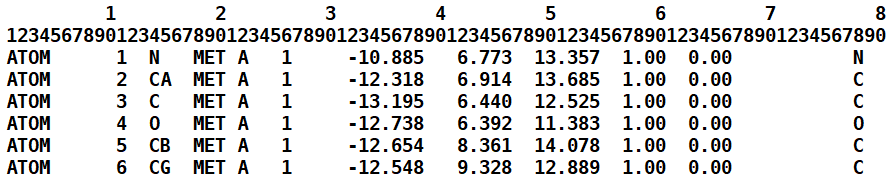
\includegraphics[width=0.95\linewidth]{atom.png}
		\end{center}
		\caption{Conjunto de entradas do tipo ATOM.}
		\label{fig:atom}
	\end{figure}
\vspace{-0.3cm}
	
	Com esse conjunto de dados, pode-se, por exemplo, esboçar uma representação gráfica de uma molécula. Existem muitos softwares compatíveis com os arquivos PDB para este fim, por exemplo, o autor deste documento implementou um a visualização de uma projeção da molécula 3D no plano z = 0, como pode-se averiguar na Figura ~\ref{fig:molproj}.
	
	\begin{figure}[H]
		\begin{center}
			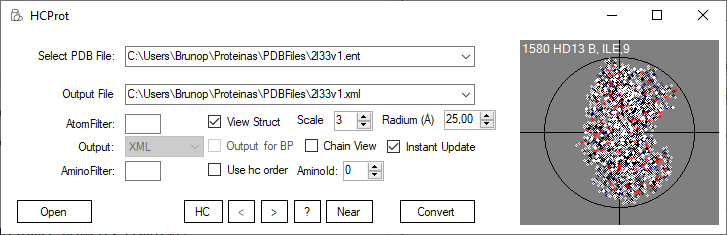
\includegraphics[width=1\linewidth]{molproj.png}
		\end{center}
		\caption{PDBReader com visualização a partir de um aquivo PDB.}
		\label{fig:molproj}
	\end{figure}
	
	
	Aqui vale um momento para uma introdução ao software desenvolvido, como parte dos resultados deste trabalho. 
	\subsubsection{\textit{Sotware PDBReader}}
	O arquivo PDB é denso, cheio de termos técnicos e pouco amigável, demandando um certo tempo para que alguém que esteja sendo introduzido nesta área se acostume com seu padrão. Por isso, surgiu a possibilidade de desenvolver uma aplicação que vise facilitar e automatizar a extração das informações das moléculas contidas nele. Este trabalho teve esse software, nomeado \textit{Protein Data Bank Reader}, como primeiro resultado prático.
	
	O software foi desenvolvido em C${^\#}$, uma linguagem de programação multiparadigma, orientada a objetos e eventos, de tipagem forte, desenvolvida pela Microsoft como parte do \textit{framework }.NET. A interface de usuário foi feita utilizando Windows Forms, como uma janela única, denominada fMain (que pode ser vista na Figura ~\ref{fig:molproj}).
	
	A aplicação pode ser usada de duas formas diferentes: Para gerar um arquivo bem formatado com os dados dos átomos contidos no arquivo PDB de entrada --- isso pode ser feito em diversos formatos, como XML, JSON, Matriz (no padrão MatLAb) e MolConf (padrão para aplicar na biblioteca Julia Language MolecularConformation.jl \cite{emersonMolConf}); Ou pode ser usado apenas como ferramenta de visualização da molécula (selecionando o \textit{checkbox} struct view).
	
	 \begin{figure}[H]
	 	\begin{center}
	 		%\hspace{-1cm}
	 		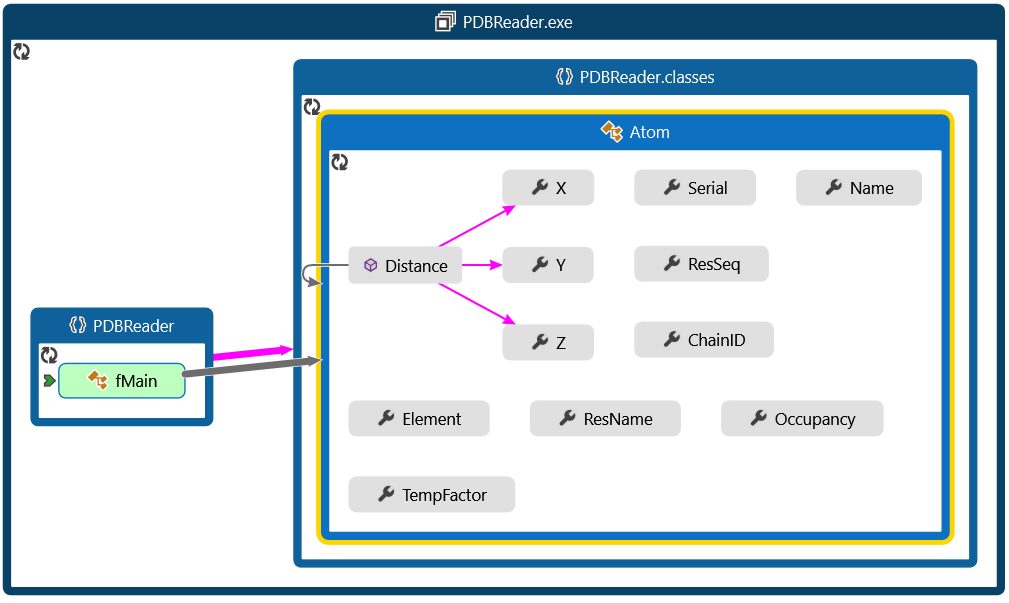
\includegraphics[width=0.9\linewidth]{classDiagram.png}
 		\end{center}
	 	\caption{Relação entre classes do PDBReader.}
	 	\label{fig:classDiagram}
	 \end{figure}
 
 	Observe na Figura ~\ref{fig:classDiagram} a existência de um conjunto de classes em \textit{PDBReader.class} que o formulário fMain utiliza. Em especial, a classe Atom, que representa um átomo, contendo todos as suas propriedades (retiradas do arquivo PDB, como as posições x, y e z) e uma função muito importante, chamada \textit{Distance}, que retorna a distância euclidiana entre dois átomos.
 	
 	O formulário fMain possui um conjunto de eventos, disparados por interações com o usuário (como mostrado na Figura ~\ref{fig:fmain}). Como pode-se perceber pelo diagrama, a grande maioria dos eventos chamam o método \textit{updateView}, que tem a função de atualizar a tela de visualização da proteína. Perceba que isso só acontece quando se está com o checkbox \textit{structView} selecionado, uma vez que o updateView só funciona nesse caso.
	
	\begin{figure}[H]
		\begin{center}
			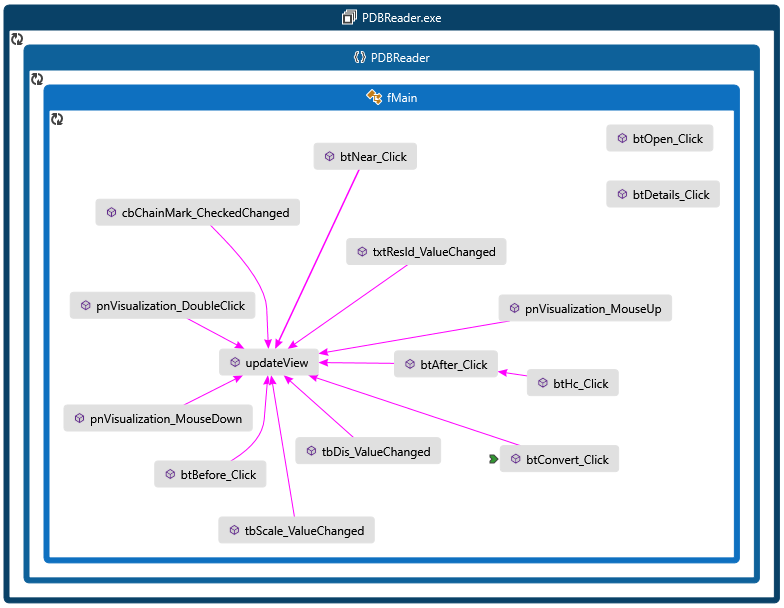
\includegraphics[width=0.86\linewidth]{fmainClassDiagram.png}
		\end{center}
		\caption{Respostas do formulário ás ações do usuário.}
		\label{fig:fmain}
	\end{figure}
	
	\subsubsection*{Brevê definição das funções do PDBReader}
	Segue abaixo uma descrição dos principais componentes do software que permitem interação com o usuário. Verifique a presença dos identificador \textit{id} de cada componente na Figura ~\ref{fig:pdbreader}, que são referenciados na Tabela ~\ref{table:pdbreader} com suas respectivas descrições.
	
	\begin{figure}[H]
		\begin{center}
			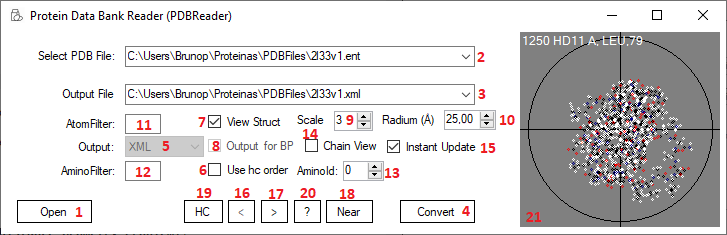
\includegraphics[width=1\linewidth]{pdbreader.png}
		\end{center}
		\caption{Interação do PDBReader.}
		\label{fig:pdbreader}
	\end{figure}
	
	\begin{table}[H]
		\hspace{-2cm}
		%\centering
		\begin{tabular}{ |c|c|c| } 
			\hline
			\textbf{id} & \textbf{Tipo} & \textbf{Descrição} \\
			\hline
			1 & Botão & Abre uma caixa de diálogo para selecionar o arquivo PDB de entrada \\\hline
			2 & Caixa de Texto & Diretório onde está o arquivo de entrada \\ \hline
			3 & Caixa de Texto & Diretório para onde será gerado o arquivo de saída\\\hline
			4 & Botão & Realiza a leitura do arquivo e faz a conversão\\\hline
			5 & Combo de Seleção & Seleciona o formato do arquivo de saída \\\hline
			6 & Caixa de Seleção & Seleciona se é para usar o Ordenação HC durante a conversão \\ \hline
			7 & Caixa de Seleção & Seleciona se o objetivo é ter uma visualização da molécula\\ \hline
			8 & Caixa de Seleção & Seleciona se será usado o padrão Branch-and-Prune na conversão\\ \hline
			9 & Entrada Numérica & Informa qual a escala para ser usada na visualização\\ \hline
			10 & Entrada Numérica & Informa o raio a ser considerado na conversão e visualização\\ \hline
			11 & Caixa de Texto & Filtrar por algum átomo específico (e.g. ``C'' para carbono)\\ \hline
			12 & Caixa de Texto & Filtrar por algum aminoácido específico (e.g. ``ALA'' para Alanina)\\ \hline
			13 & Entrada Numérica & Se > 0 filtra para o aminoácido de identificador específico\\ \hline
			14 & Caixa de Seleção & Se selecionado pinta de rosa todas as cadeias que não forem a primeira\\ \hline
			15 & Caixa de Seleção & Se deseja que o software atualize o painel sempre que houver alterações.\\ \hline
			16 & Botão & Permite movimentação entre átomos, centraliza a tela no átomo anterior\\ \hline
			17 & Botão & Permite movimentação entre átomos, centraliza a tela próximo átomo\\ \hline
			18 & Botão & Centraliza o painel no átomo com menor distância para o atual\\ \hline
			19 & Botão & Tenta percorrer o aminoácido atual usando a ordem HC de forma empírica\\ \hline
			20 & Botão & Abre uma janela com informações sobre o átomo atual e os próximos\\ \hline
			21 & Painel Visual & Centraliza o painel em um átomo clicando duas vezes nele\\\hline
		\end{tabular}
		\caption{Descrição dos componentes do software.}
		\label{table:pdbreader}
	\end{table}

	Por exemplo, pode-se estudar apenas o segundo aminoácido (Alanina) da proteína Calcyclin (codigo PDB 1A03) --- uma proteína do tipo ligante de cálcio --- apenas setando o AminoId (componente 13 da Figura ~\ref{fig:pdbreader}) para 2 e selecionando o View Sctruct (componente 7). Também podemos alterar a escala de exibição (componente 9) e a distância radial de visão (componente 10), para facilitar a visualização nessa dimensão pequenina. O resultado se vê na Figura ~\ref{fig:exemploView}.
	
	\begin{figure}[H]
		\hspace{-1.3cm}
		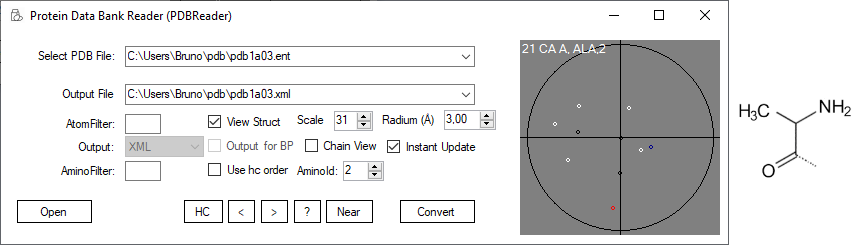
\includegraphics[width=1.2\linewidth]{exemploView.png}
		\caption{Visualização de uma Alanina utilizando o PDBReader.}
		\label{fig:exemploView}
	\end{figure}
	
	\newpage
	\section{\textit{Molecular Distance Geometry Problem}}
	Até o momento, provavelmente, já deve estar mais que claro a importância de se estudar a estrutura tridimensional de proteínas e a grande complexidade relacionada a esta tarefa. De fato, a bioquímica é um universo de estudos imenso e, se não tomarmos cuidado, facilmente nos perderemos entre seus labirintos. Porém, a partir daqui voltaremos nosso olhar para uma perspectiva um pouco mais matemática, o que nos dá uma capacidade de abstração elevada.
	
	Sempre perdemos alguma coisa quando trazemos um problema da vida real para um modelo matemático. Com a experiência, adquirimos a habilidade de optar pelas hipóteses corretas para solucionar o problema mais próximo possível do real, porém, ao fazê-lo, essas hipóteses podem dificultar demasiadamente a busca por uma solução. Esse é um dilema recorrente na matemática aplicada.
	 
	Nesse capitulo, estudaremos algumas definições importantes que nos darão base e estrutura para discutir sobre as possíveis hipóteses do problema, onde tentaremos construir, juntos, a sua real definição.  
	
	\subsection{Geometria de Distâncias}
	O principal conteúdo de estudo da Geometria de Distâncias, como o próprio nome sugere, rodeia a ideia de distância entre objetos de determinada estrutura geométrica. Assim, o problema fundamental da Geometria de Distâncias consiste em determinar um conjunto de pontos, pertencentes a um espaço geométrico, com base nas distâncias conhecidas entre tais pontos. Note que nem sempre sabemos todas as distâncias entre todos os pontos.
	
	O surgimento da Geometria de Distâncias se deu por volta de 1928, com o matemático Karl Menger, que caracterizou uma série de conceitos geométricos (e.g. congruência; conjuntos convexos) em termos de distâncias \cite{carlileGDandAplications}. Entretanto, somente em 1953, com Leonard Blumenthal, que a Geometria de Distâncias tornou-se uma nova área de conhecimento \cite{carlileBook31Coloquio}. E foi graças a Yemini, em 1978, que o problema fundamental de Geometria de Distâncias foi enunciado.
	
	\begin{center}
		\begin{minipage}{0.9 \linewidth}
			\textbf{Distance Geometry Problem (DGP):} Dado $K \in \mathbb{Z}_{+}$ e um grafo simples e não-direcionado $G = (V,E)$ cujas arestas são ponderadas pelos valores da função não-negativa $d: E \longrightarrow \mathbb{R}_{+}$, determine se existe imersões $x:V \longrightarrow \mathbb{R}^{K}$ (realizações do grafo) tais que
			\begin{equation}
			\forall \{u,v\} \in E, \hspace{0.5cm} \left\| x_{u} - x_{v} \right\| = d_{u,v}. \label{eq:DGP}
			\end{equation}
		\end{minipage}
	\end{center}
	
	Perceba a grande beleza que emana desse problema inverso. Uma das suas características mais interessantes é sua simplicidade --- tem como entrada apenas um conjunto de distâncias entre pontos não localizados e procura-se localizá-los ---, que o leva a ser aplicado em muitas diferentes áreas do conhecimento \cite{carlileGDandAplications}. 
	
	Tendo em mente nosso problema fundamental, podemos ajustar nossos dados moleculares para aplicá-lo.
	
	\subsection{Representações de Átomos em Coordenadas\label{sec:bi}}
	Como as partículas que estamos interessados estão localizadas no espaço tridimensional, podemos representa-las utilizando coordenadas cartesianas tridimensionais $x_1, ...,x_n \in\mathbb{R}^3$, onde $x_n$ é a \textit{realização} do n-ésimo átomo da molécula analisada. 
	
	Além da utilização das coordenadas cartesianas, também podemos usar outro sistema de coordenadas, mais condizente com os dados que temos a priori sobre a molécula --- rever Figura ~\ref{fig:rama}. Tal sistema denomina-se \textit{coordenadas internas} (e tem forte relação com as coordenadas esféricas).
	
	As coordenadas internas de uma proteína são definidas pela distância entre os átomos $d_{1,2}, ..., d_{n - 1,n}$, pelo ângulo planar $\theta_{1,3}, ...,\theta_{n - 2,n}$ (formados por 3 átomos consecutivos) e pelos ângulos de torção $\omega_{1,4}, ..., \omega_{n-3,n}$ (formado por 4 átomos consecutivos), conforme ilustrado na Figura ~\ref{fig:angulos}. O ângulo de torção é definido entre os planos formados pelos átomos $i-3,i-2,i-1$ e$i-2,i-1,i$, respectivamente. Assim, temos que $\omega$ varia no intervalo $[0,2\pi]$ e $\theta$ de $[0,\pi]$ --- assim como em um sistema de coordenadas esféricas --- e também já vimos que as distâncias entre os átomos unidos por ligações covalentes são da ordem de 1,5\AA. 
	
	\begin{figure}[H]
		\begin{center}
			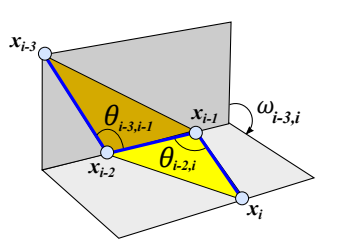
\includegraphics[width=0.6\linewidth]{Capturar.PNG}
		\end{center}
		\caption{Ângulos planos e de torção \cite{carlileBook31Coloquio}}
		\label{fig:angulos}
	\end{figure}
	
	Pode-se obter facilmente os ângulos planos pela \textit{Lei dos Cossenos}, tendo em vista que conhece-se todas as distâncias que, por construção, representam os lados do triângulo --- para mais detalhes, recorrer ao Apêndice A. Porém, descobrir o ângulo de torção associado (também chamado de ângulo diedral) pode se mostrar um grande problema. 
	
	O cosseno de um ângulo diedral pode ser dado em função de distâncias euclidianas e ângulos planos \cite{carlileTese}. Sejam $x_i, x_j, x_k, x_l \in \mathbb{R}^3$ quaisquer quatro átomos consecutivos com coordenadas ($x_{i_1}, x_{i_2}, x_{i_3}$), ($x_{j_1}, x_{j_2}, x_{j_3}$), ($x_{k_1}, x_{k_2}, x_{k_3}$) e ($x_{l_1}, x_{l_2}, x_{l_3}$), respectivamente; Também $r_{ab}$, com $a,b \in \{i,j,k,l\}$ as distâncias entre os átomos $x_a$ e $x_b$; e por último $\theta_{ijk}$, o ângulo definido pelos átomos $x_i, x_j, x_k$ e $\theta_{kji}$, o ângulo definido pelos átomos $x_k, x_j, x_i$. Então, o cosseno do ângulo diedral $\omega_{ijkl}$ é dado por:
	
	\begin{equation}
	\cos(\omega_{ijkl}) = \frac{r^2_{ij} + r^2_{jl} - 2r_{ij}r_{jl}\cos(\theta_{ijk})\cos(\theta_{kjl}-r^2_{il})}{2r_{ij}r_{jl}\mbox{sen}(\theta_{ijk})\mbox{sen}(\theta_{kjl})}. \label{eq:cosOmega}
	\end{equation}    
	
	Porém, não temos como definir exatamente o seno desse ângulo. Só podemos fazer $\mbox{sen}(\omega_{ijkl}) = \pm\sqrt{1 - \cos(\omega_{ijkl})^2} \label{eq:senOmega}$. Mas vamos deixar esse problema do ângulo de torção para outra hora --- por enquanto supomos que temos os valores exatos de $\omega_{ijkl}$.
	
	Por tanto, conseguimos definir todo o problema a partir das coordenadas internas. Como nosso objetivo é obter as posições tridimensionais de cada átomo, nosso problema se restringiu em transformar as coordenadas internas em cartesianas. Para isso, utiliza-se uma série de operações lineares que estão descritas pelas matrizes abaixo.
	
	Consideremos que as coordenadas do ponto $x_{i} \in\mathbb{R}^3,i= 1, ...,n $ são dadas por $(x_{i1},x_{i2},x_{i3})$, temos:
	
	$$
	\begin{bmatrix}
	x_{i1}\\ 
	x_{i2}\\ 
	x_{i3}\\ 
	1
	\end{bmatrix}
	= B_{1}B_{2}\cdots B_{i}\begin{bmatrix}
	0\\ 
	0\\ 
	0\\ 
	1
	\end{bmatrix},
	$$
	onde
	$$
	B_1\: =\:
	\begin{bmatrix}
	1 & 0 & 0 & 0\\ 
	0 & 1 & 0 & 0\\ 
	0 & 0 & 1 & 0\\ 
	0 & 0 & 0 & 1
	\end{bmatrix},\:\:\:
	\: B_2\: =\:
	\begin{bmatrix}
	-1 & 0 & 0 & -d_{1,2}\\
	0 & 1 & 0 & 0\\ 
	0 & 0 & -1 & 0\\ 
	0 & 0 & 0 & 1
	\end{bmatrix},
	$$
	$$
	B_3\:=\:
	\begin{bmatrix}
	-\cos\theta_{1,3} & -\mbox{sen}\theta_{1,3} & 0 & -d_{2,3}\cos\theta_{1,3}\\ 
	\mbox{sen}\theta_{1,3} & -\cos\theta_{1,3} & 0 & d_{2,3}\mbox{sen}\theta_{1,3}\\ 
	0 & 0 & 1 & 0\\ 
	0 & 0 & 0 & 1
	\end{bmatrix}
	$$
	e
	$$
	B_i\:=\:
	\begin{bmatrix}
	-c_{\theta_{i}} & -s_{\theta_{i}} & 0 & -d_{i-1,i}c_{\theta_{i}}\\ 
	s_{\theta_{i}}c_{\omega_{i}} & -c_{\theta_{i}}c_{\omega_{i}}
	& -s_{\omega_{i}} & d_{i-1,i}s_{\theta_{i}}c_{\omega_{i}}\\ 
	s_{\theta_{i}}s_{\omega_{i}} & -c_{\theta_{i}}s_{\omega_{i}} & c_{\omega_{i}} & d_{i-1,i}s_{\theta_{i}}s_{\omega_{i}}\\ 
	0 & 0 & 0 & 1
	\end{bmatrix}
	$$
	dado $s_{\theta_{i}}=\mbox{sen} (\theta_{i-2, i}),\: c_{\theta_{i}}=\cos (\theta_{i-2, i}),\: s_{\omega_{i}}=\mbox{sen} (\omega_{i-3, i}),\: c_{\omega_{i}}=\cos (\omega_{i-3, i})$. Em $B_i$, $i=4, ..., n$.
	
	
	Perceba que $B_i$ (chamada \textit{Matriz de Torção}) é a matriz que engloba todas as operações necessárias para encontrar a i-ésima realização do i-ésimo átomo da molécula, tendo conhecimento de todas as matrizes $B_j$ $\forall j < i$. Como é de grande importância o entendimento de tais operações que formam a $B_i$, deixa-se o Apêndice B para esta discussão.
	
	Note também que fixando os comprimentos das ligações covalentes $d_{1,2},d_{2,3}$ e o valor do ângulo plano $\theta_{1,3}$, os três primeiros átomos terão as coordenadas dadas por
	$$
	x_1\:=\:
	\begin{bmatrix}
	0\\ 
	0\\  
	0
	\end{bmatrix},\:\:\:
	x_2\:=\:
	\begin{bmatrix}
	-d_{1,2}\\ 
	0\\  
	0
	\end{bmatrix},\:\:\:
	x_3\:=\:
	\begin{bmatrix}
	-d_{1,2}+d_{2,3}\cos\theta_{1,3}\\ 
	d_{2,3}\mbox{sen}\theta_{1,3}\\  
	0
	\end{bmatrix}.
	$$
	
	Dadas essas três realizações dos primeiros átomos, fixamos a base do sistema, evitando estruturas obtidas por meio de rotações e translações a partir de uma mesma estrutura.	
	
	Além dos dados teóricos sobre as estruturas dos aminoácidos, também teremos dados de distâncias entre átomos dadas de forma experimental, através de experimentos de RMN.
	
	\subsection{Ressonância Magnética Nuclear}
	A ressonância magnética nuclear é um processo físico que analisa a interação da radiação eletromagnética com a matéria. Neste experimento é escolhida uma faixa de radiofrequência para bombardear uma amostra que está imersa em um campo magnético bastante intenso. Dependendo da radiofrequência utilizada, alguns núcleos atômicos irão absorver energia e outros não. Caso atinja-se uma frequência exata de ressonância dentro destes núcleos atômicos, é possível medir essa ressonância como um sinal de radiofrequência enviado dos núcleos atômicos --- para calcular distâncias entre átomos próximos, com distâncias menores que 5\AA. No nosso problema, a frequência utilizada é para a ressonância dos núcleos de hidrogênio e um computador capta essas respostas eletromagnéticas dos núcleos atômicos para utilizar como dados do problema. \cite{RMNBookIntroduction}
	
	Assim, esse procedimento fornece vários \textit{intervalos} de distâncias possíveis relativas associadas a átomos de hidrogênio próximos (sendo que por vezes também 
	é capaz de captar átomos de um isótopo específico de carbono, devido a proximidade de sua frequência com a do hidrogênio), esses intervalos também são chamados de \textit{distancias intervalares}. Pode-se representar essas distancias intervalares matematicamente por intervalos de números reais $[d_{i,j}^i, d_{i,j}^f]$ . Isto é, existe um real $d_{i,j}$ que representa a distância real tal que
	
	$$ 0 \leq d_{i,j}^i \leq d_{i,j} \leq d_{i,j}^f$$
	
	\subsection{Modelagem Matemática}
	Quando um pesquisador de outra área se depara com um problema que não consegue resolver e precisa recorrer aos matemáticos, quase sempre se torna uma tarefa muito complicada para quem for tentar desenvolver o problema. Não pela complexidade matemática do assunto, isto os matemáticos dominam. A dificuldade está em entender o problema de outras áreas e, como se por ironia, resolve-los. Este é um fardo que se tem de carregar quando se escolhe trabalhar com uma ciência que é utilizada por tantas outras. No entanto, por sorte, os matemáticos são apaixonados por interpretar, modelar e resolver problemas.
	
	A boa interpretação de um problema de matemática aplicada deve se ater a algumas perguntas importantes:
	\begin{itemize}
		\item \textbf{Quais são as hipóteses?} Ou seja, fatos dos quais devemos nos basear e nos limitar para propor, de forma dialética, uma solução para o problema. Nos importaremos com seis hipóteses que advém de informações já discutidas aqui:
		\begin{description}
			\item[Hipótese 1:]as distâncias fornecidas pelos experimentos de RMN estão associados a pares de átomos conhecidos: nós sabemos a quais átomos as distâncias se referem (isso não é bem verdade, mas supomos que seja assim para desenvolver o problema);
			\item[Hipótese 2:]todos os átomos da molécula da proteína cuja estrutura 3D queremos calcular são conhecidos: conhecermos a estrutura química da molécula;
			\item[Hipótese 3:]todos os átomos da molécula de proteína estão ligadas a algum átomo cuja distância é conhecida: não há átomos soltos, afinal, se existisse, seria outra molécula;
			\item[Hipótese 4:]existe uma ordem, dada a priori, entres os átomos da cadeia principal da proteína cuja estrutura 3D queremos calcular: conhecemos o esqueleto padrão --- backbone ---, formado de aminoácidos, da molécula de proteína examinada;
			\item[Hipótese 5:]as distâncias entre os átomos de uma molécula de proteína separados por duas ligações covalentes são conhecidas: existem esses resultados na literatura;
			\item[Hipótese 6:]as distâncias fornecidas pela RMN são representandos por intervalos de números reais que contêm o valor correto associado.
		\end{description}
		
		\item \textbf{Qual resultado deseja-se obter?} De forma simplificada, qual é nossa \textit{tese}? Dificilmente se chega no lugar ideal se não há o conhecimento da direção a seguir. Cabe-se uma definição formal dos nossos objetivos:
		\begin{center}
			\begin{minipage}{0.9 \linewidth}
				Deve-se determinar os pontos $x_{i}\in\mathbb{R}^3$, $i = 1, \dots, n$ ($n$ é o número de átomos da molécula), satisfazendo as equações
				$$\|x_i -x_j\|=d_{ij} , \forall {i,j} \in E
				$$
				\textit{onde} $E \subset \{1, ...,n\} \times \{1, ...,n\}$ e $d_{ij}$ \textit{são os valores de distâncias fornecidas pela RMN.}
			\end{minipage}
		\end{center}
		
		Tentar resolver os sistemas de equações acima parece não ser uma boa ideia, já que existem evidências de que não seja possível obter uma fórmula fechada para isso \cite{carlileBook31Coloquio}. Podemos até tentar resolver numericamente, porém as soluções seriam infinitas para as equações.
		
		A abordagem mais usual é a representação do problema usando otimização. Para isso devemos  resolver todas as equações do problema. Podemos, dessa maneira, considerar uma única expressão com todas elas, dada por
		$$ f(x_1, ...,x_n) \equal \sum_{(i,j) \in E} (\|x_i - x_j\| - d_{ij})^2
		$$
		
		Para resolvermos tal otimização, basta encontrar valores de $x_i \in \mathbb{R}^3$, $i = 1, ..., n$, tal que $f(x_1, ...,x_n)=0.$ Assim temos
		$$ \min_{x_i \in\mathbb{R}^n} f(x_1, ...,x_n).
		$$
		
		A dificuldade nesse caso está em encontrar o mínimo global, pois existem vários mínimos locais e estes\textit{ crescem exponencialmente com a  quantidade de átomos da molécula}. Outro ponto delicado é que pode ser muito complicado distinguir um mínimo local de um global, uma vez que os métodos de otimização continua só se referem a informações locais. Isso tudo torna o problema muito custoso para resolver.
	\end{itemize}
	
	\subsubsection{MDGP: Uma definição formal}
	Agora que temos uma boa base, vamos definir o Problema de Geometria de Distâncias Moleculares formalmente \cite{carlileBook31Coloquio}.
	
	\begin{center}
		\begin{minipage}{0.9 \linewidth}
			\textbf{Molecular Distance Geometry Problem:} Dado um grafo simples não-direcionado $G=(V,E)$, de modo que suas arestas sejam valoradas por uma função não-negativa $d:E\rightarrow\mathbb{R_+}$, considere a seguinte aplicação:
			$$x:V\rightarrow\mathbb{R}^3
			$$
			De modo que para todo $\{u,v\}\in E$ temos:
			$$\|x(u)-x(v)\|=d({u,v})
			$$
		\end{minipage}
	\end{center}

	É fácil ver que essa se trata de uma especificação do DGP, onde $k = 3$. Logo, nossa tarefa é encontrar uma aplicação $x$ que satisfaça todas as distâncias e dados do grafo que temos. Esta função é denominada \textit{realização} de $G$. Quando a realização satisfaz todas as equações da forma "$\|x(u)-x(v)\|=d({u,v})$", dizemos que ela é uma \textit{realização válida}.
	
	
	\subsection{Modelagem Computacional}
	
	Uma vez que existe uma introdução a modelagem matemática do problema, pode-se pensar em uma abordagem computacional. Não é segredo para ninguém que a computação veio e vem melhorando muito a forma como se faz matemática, introduzindo novas ferramentas e campos de estudo de grande importância. Vamos utilizar dessa evolução para a solução desse problema que, de outra forma, não seria viável. Na verdade, uma das dúvidas que estamos motivados a responder aqui é se, mesmo com toda nossa capacidade computacional atual, o problema tem uma solução viável. Definiremos melhor adiante o que é uma solução dita \textit{viável}. 
	
	\subsubsection*{Dados de Entrada e Saída}
	É um paradigma de computação se preocupar em deixar claro quais dados devem ser de entrada (\textit{input}), para serem utilizados, processados, modificados e todo o resto que necessitar para gerar os dados de saída (\textit{output}).
	
	Existem dois tipos de dados que serão tratados aqui, os dados \textit{teóricos} e os dados \textit{reais}. Todos os dados reais que utilizamos são provenientes dos experimentos de RMN. Já os teóricos vem de conhecimento da Química, Física e Biologia.
	
	\begin{description}
		\item{Dados de Entrada \cite{carlileBook31Coloquio}}:
		\begin{itemize}
			\item quantidade de átomos: $n$;
			\item sequências de átomos:
			$$N^1,C^{1}_{\alpha},C^1,N^2,C^{2}_{\alpha},C^2, ...,N^{n/3},C^{n/3}_{\alpha},C^{n/3};
			$$
			\item distância entre os átomos separados por uma ligação covalente: $\{d_{1,2},d_{2,3}, ...,d_{n-1,n}\}$, onde $i = 2, ..., n;$
			\item distância entre os átomos separados por duas ligações covalentes: $\{d_{1,3},d_{2,4}, ...,d_{n-2,n}\}$, $i=3, ..., n;$
			\item distância entre átomos próximos, com no máximo 5 \AA, fornecidas pela RMN \textit{- único dado de entrada real};
		\end{itemize}
		\item{Dados de Saída:}
		\begin{itemize}
			\item posições $x_1, ...,x_n \in\mathbb{R}^3$ dos $n$ átomos da proteína.
		\end{itemize}
	\end{description}
	
	Como as distâncias fornecidas pela RMN são um dado real, não são um valor exato. Dados reais são incertos, dependem de muitas variáveis, como a precisão da ferramenta que a mediu, o tipo de medida, quantas vezes fora medido, entre outras coisas. Esta incerteza é calculada e pode-se saber mais sobre em \cite{EstatisticaTratamentoDeDados}.
	
	\subsubsection*{Complexidade do MDGP}
	É de extrema importância verificarmos o custo computacional de se tentar resolver o MDGP, pois, só com esta analise, pode-se dizer se o problema tem ou não uma solução viável. Caso não tenha, o trabalho pode ser encerrado por aqui. De nada nos adianta solução que não pode ser calculada.
	
	Para poder calcular o custo computacional de uma solução matemática, deve-se verificar quantas vezes o ``\textit{núcleo}'' do programa é computado, ou seja, se verifica quantas vezes a operação central do programa é realizada. Caso for realizada apernas uma vez, dizemos que o custo é baixo. Caso essa quantidade cressa proporcionalmente a medida que aumentamos os dados de entrada do problema (por exemplo, a medida que aumentamos a quantidade $n$ de átomos da molécula), então dizemos que a dificuldade é linear. Para mais detalhes sobre custo computacional, leia \cite{ComplexidadeComp}. Resolvemos, então, um MDGP simples --- retirado de \cite{carlileBook31Coloquio} --- e verificamos qual seria seu custo.
	
	Considere um MDGP restrito ao plano, onde temos um grafo $G = (V(G), E(G))$ tal que $V(G)=\{u, v, r, s\}$ e $E(G)=\{\{u,v\}, \{u, r\}, \{v, r\}, \{v, s\}, \{r, s\}, \{u, s\}\}$. Fixando \textit{u, v, r} e \textit{s}, ou seja, determinando $ x_{u}, x_{v},x_{r} \in\mathbb{R}^2$ de tal modo que $\|x_{u} - x_{v}\|= d_{uv}$,  $\|x_{u} - x_{r}\|= d_{ur}$ e $\|x_{v} - x_{r}\|= d_{vr}$, podemos montar o  seguinte sistema quadrático:
	$$ \|x_{s} - x_{u}\|= d_{us} $$$$ \|x_{s} - x_{v}\|= d_{vs} $$$$ \|x_{s} - x_{r}\|= d_{rs} $$
	Elevando os termos ao quadrado,
	$$\|x_{s}\|^{2} - 2(x_{s}.x_{u}) + \|x_{u}\|^{2} = d_{us}^{2}$$
	$$\|x_{s}\|^{2} - 2(x_{s}.x_{v}) + \|x_{v}\|^{2} = d_{vs}^{2}$$
	$$\|x_{s}\|^{2} - 2(x_{s}.x_{r}) + \|x_{r}\|^{2} = d_{rs}^{2}$$
	subtraindo a primeira equação das outras duas, temos:
	$$2(x_{s}.x_{v}) - 2(x_{s}.x_{u}) = \|x_{v}\|^{2} - \|x_{u}\|^{2} + d_{us}^{2} - d_{vs}^{2}$$
	$$2(x_{s}.x_{r}) - 2(x_{s}.x_{u}) = \|x_{r}\|^{2} - \|x_{u}\|^{2} + d_{us}^{2} - d_{rs}^{2}$$
	Colocando $x_{s}$ em evidência para ficar claro as incógnitas
	$$2(x_{v} - x_{u})x_{s} = \|x_{v}\|^{2} - \|x_{u}\|^{2} + d_{us}^{2} - d_{vs}^{2}$$
	$$2(x_{r} - x_{u})x_{s} = \|x_{r}\|^{2} - \|x_{u}\|^{2} + d_{us}^{2} - d_{rs}^{2}$$
	Por tanto, temos um sistema linear $Ax = b$, onde
	$$
	A = 2\begin{bmatrix}
	x_{v1} - x_{u1} & x_{v2} - x_{u2}\\
	x_{r1} - x_{u1} & x_{r2} - x_{u2}
	\end{bmatrix},
	$$
	$$
	b = \begin{bmatrix}
	\|x_{v}\|^{2} - \|x_{u}\|^{2} + d_{us}^{2} - d_{vs}^{2}\\
	\|x_{r}\|^{2} - \|x_{u}\|^{2} + d_{us}^{2} - d_{rs}^{2}
	\end{bmatrix},
	$$
	e
	$$
	x = \begin{bmatrix}
	x_{s1}\\
	x_{s2}
	\end{bmatrix}.
	$$
	
	Se a matriz \textit{A} for inversível, temos uma única solução $x^{*} = A^{-1}b$. Logo, podemos concluir que se o grafo \textit{G} de um MDGP for completo, podemos resolver o problema através da resolução de $n$ sistemas lineares, sendo $n$ proporcional ao número de vértices (átomos da molécula). Diz-se, então, que o problema pode ser resolvido em tempo \textit{linear}.
	
	No entanto, isso não acontece. Sabemos que o grafo molecular não é completo pois algumas distâncias não são informadas, assim, teremos apenas parte do grafo. 
	
	Admitindo que todas as distâncias dadas são valores \textit{precisos} e que certamente representam as distâncias entre os átomos, o problema então terá uma solução. Para encontrarmos a solução devemos achar o mínimo global discutido na modelagem matemática, que, como vimos anteriormente, é inviável. A quantidade de mínimos locais cresce exponencialmente com a quantidade de vértices. Ou seja, o custo computacional para resolver um MDGP onde, suponha, todas as distâncias da RMN são realmente precisas, pode ser proporcional a $2^n$, onde $n$ é a quantidade de átomos. O que faz esse problema entrar na classificação \textit{NP-difícil}. \cite{ComplexidadeComp}
	
	Por tanto, precisamos encontrar outra abordagem para solucionar nosso problema. É assim o processo cientifico. Nosso próximo passo será tentar garantir que, ao menos, não tenhamos uma quantidade não enumerável de soluções do problema.
	
	\subsection{Estudando o Conjunto Solução de um MDGP}
	Com base no que temos, podemos analisar condições para garantir a finitude do conjunto solução do MDGP --- conforme em \cite{carlileBook31Coloquio}. A cardinalidade do conjunto solução de um MDGP (elementos são funções) pode ajudar na solução do problema. Sabemos que um MDGP pode ter conjunto solução vazio, solução única ou ser não-enumerável. Para essa analise, consideremos o mesmo problema da seção anterior, porém, nesse caso, os vértices não estão restritos ao plano. Temos, então, um MDGP com $V=\{u, v, r, s\}$ e $E=\{\{u,v\}, \{u, r\}, \{v, r\}, \{v, s\}, \{r, s\}, \{u, s\}\}$. Fixamos \textit{u, v, r} e \textit{s}; obtemos o mesmo sistema quadrático:
	$$
	\|x_{s} - x_{u}\|= d_{us}
	$$
	$$
	\|x_{s} - x_{v}\|= d_{vs}
	$$
	$$
	\|x_{s} - x_{r}\|= d_{rs}
	$$
	Fazendo o mesmo procedimento anterior de elevar ao quadrado e subtrair a primeira das outras duas, obtemos:
	$$
	2(x_{v} - x_{u})x_{s} = \|x_{v}\|^{2} - \|x_{u}\|^{2} + d_{us}^{2} - d_{vs}^{2}
	$$
	$$
	2(x_{r} - x_{u})x_{s} = \|x_{r}\|^{2} - \|x_{u}\|^{2} + d_{us}^{2} - d_{rs}^{2}
	$$
	Até agora, nada mudou, porém, agora escrevendo explicitamente, temos:
	$$
	\begin{bmatrix}
	x_{v1} - x_{u1} & x_{v2} - x_{u2} & x_{v3} - x_{u3}\\
	x_{r1} - x_{u1} & x_{r2} - x_{u2} & x_{r3} - x_{u3}
	\end{bmatrix}
	\begin{bmatrix}
	x_{s1}\\
	x_{s2}\\
	x_{s3}
	\end{bmatrix} =
	\frac{1}{2}\begin{bmatrix}
	\|x_{v}\|^{2} - \|x_{u}\|^{2} + d_{us}^{2} - d_{vs}^{2}\\
	\|x_{r}\|^{2} - \|x_{u}\|^{2} + d_{us}^{2} - d_{rs}^{2}
	\end{bmatrix}
	$$
	Ou seja, não temos mais uma matriz $2 \times 2$, mas  sim, uma matriz $2 \times 3$.
	
	Reescrevendo o sistema de outra maneira
	$$
	\begin{bmatrix}
	x_{s1}\\
	x_{s2}
	\end{bmatrix} +
	\begin{bmatrix}
	x_{v3} - x_{u3}\\
	x_{r3} - x_{u3}
	\end{bmatrix}
	\begin{bmatrix}
	x_{s3}
	\end{bmatrix} =
	\frac{1}{2} \begin{bmatrix}
	\|x_{v}\|^{2} - \|x_{u}\|^{2} + d_{us}^{2} - d_{vs}^{2}\\
	\|x_{r}\|^{2} - \|x_{u}\|^{2} + d_{us}^{2} - d_{rs}^{2}
	\end{bmatrix}
	$$
	E supondo que a matriz
	$$
	A = \begin{bmatrix}
	x_{v1} - x_{u1} & x_{v2} - x_{u2}\\
	x_{r1} - x_{u1} & x_{r2} - x_{u2}
	\end{bmatrix}
	$$
	seja inversível, obtemos
	$$
	\begin{bmatrix}
	x_{s1}\\
	x_{s2}
	\end{bmatrix} =
	\frac{1}{2} A^{-1} \begin{bmatrix}
	\|x_{v}\|^{2} - \|x_{u}\|^{2} + d_{us}^{2} - d_{vs}^{2}\\
	\|x_{r}\|^{2} - \|x_{u}\|^{2} + d_{us}^{2} - d_{rs}^{2}
	\end{bmatrix} -
	A^{-1}\begin{bmatrix}
	x_{v3} - x_{u3}\\
	x_{r3} - x_{u3}
	\end{bmatrix}
	\begin{bmatrix}
	x_{s3}
	\end{bmatrix}
	$$
	isso agora implica que não temos mais solução, pois, para cada valor de $x_{s3} \in\mathbb{R}$, obtemos valores para $x_{s1}$ e $x_{s2}$.
	
	Para encontramos uma solução, devemos retornar ao sistema quadrático e resolver uma equação do sistema linear acima.
	
	Geometricamnete, temos a interseção de uma reta, dada por
	$$
	\begin{bmatrix}
	x_{s1}\\
	x_{s2}
	\end{bmatrix} =
	A -
	B
	\begin{bmatrix}
	x_{s3}
	\end{bmatrix}
	$$
	onde
	$$
	A = \frac{1}{2} \begin{bmatrix}
	x_{v1} - x_{u1} & x_{v2} - x_{u2}\\
	x_{r1} - x_{u1} & x_{r2} - x_{u2}
	\end{bmatrix}^{-1} 
	\begin{bmatrix}
	\|x_{v}\|^{2} - \|x_{u}\|^{2} + d_{us}^{2} - d_{vs}^{2}\\
	\|x_{r}\|^{2} - \|x_{u}\|^{2} + d_{us}^{2} - d_{rs}^{2}
	\end{bmatrix} 
	$$
	$$
	B = \begin{bmatrix}
	x_{v1} - x_{u1} & x_{v2} - x_{u2}\\
	x_{r1} - x_{u1} & x_{r2} - x_{u2}
	\end{bmatrix}^{-1}
	\begin{bmatrix}
	x_{v3} - x_{u3}\\
	x_{r3} - x_{u3}
	\end{bmatrix}
	\begin{bmatrix}
	x_{s3}
	\end{bmatrix}
	$$
	e uma esfera tal que
	$$
	\|x_{s} - x_{u}\|= d_{us}
	$$
	resultando em 3 possibilidades: conjunto vazio (a reta não intersepta a esfera); apenas um ponto (a reta é tangente à esfera); dois pontos (a reta é secante à esfera).
	
	A discussão sugere dois aspectos importantes sobre a finitude:
	
	\begin{enumerate}
		\item Para cada vértice $s\in V$ a ser realizado em $\mathbb{R}$, devem existir arestas ${u, s}, {v, s}, {r, s} \in E$ tais que os vértices $u, v, r \in V$ já tenham sido realizados, para que se possa gerar um sistema quadrático, com $x_{s} \in\mathbb{R}^{3}$ como única incógnita, dado por
		$$
		\|x_{s} - x_{u}\|= d_{us}
		$$
		$$
		\|x_{s} - x_{v}\|= d_{vs}
		$$
		$$
		\|x_{s} - x_{r}\|= d_{rs}
		$$
		\item Para que esse sistema tenha no máximo duas soluções, a matriz linear do sistema obtido subtraindo uma equação das outras duas deve ter posto completo.
	\end{enumerate}
	
	As duas informações cruciais, relacionadas ao vértice $s\in V$, são:
	\begin{itemize}
		\item Existem $u, v, r \in V$ tais que $\{u, s\}, \{v, s\}, \{r, s\}\subset E$,
		\item $x_{u}, x_{v}, x_{r} \in\mathbb{R}^{3}$ fazem parte de uma realização \textit{parcial} válida. 
	\end{itemize}
	
	A ideia que conecta os pontos anteriores está ligada ao conceito de \textit{ordem nos vértices} do grafo $G = (V, E, d)$ do MDGP. Se existir uma ordem dos vértices que satifaz as condições 1 e 2 acima, podemos garntir, a menos de rotações e translações, que o cojunto solução do problema é finito.
	
	Relembremos que resolver um MDGP é conseguir uma realização válida $x: V \rightarrow\mathbb{R}^{3}$ do grafo associado, o que implica, por sua vez, definir um ponto $x_{s}\in\mathbb{R}^3$, para cada $s\in V$, satisfazendo todas as equações do sistema
	$$
	\forall {u, v}\in E, \|x_{u} - x_{v}\| = d_{uv}.
	$$
	Portanto uma solução do problema pode ser representada, então, como um elemento do $\mathbb{R}^{3\|V\|}$
	
	\subsection{Ordenação Conveniente dos Vértices \label{sec:hc}}
	Ótimo, estamos progredindo. Caso exista uma ordenação que respeite essas condições, podemos tornar a busca por uma solução para o problema factível. Porém, encontrar tal ordem, no geral, não é trivial e depende muito da natureza do problema. Encontrar essa ordem trata-se do $\emph{Problema da Ordem de Vértices Discretizáveis}$ --- ou simplesmente DVOP (do inglês, \textit{Discretization Vertex Order Problem}). Segue sua definição formal:
	
	\begin{center}
		\begin{minipage}{0.9 \linewidth}
			\textbf{\textit{Discretization Vertex Order Problem}:} Dado um grafo simples não direcionado $G = (V, E)$ e um escalar positivo $K$, estabelecer se existe uma ordem $<$ em $V$ tal que: 
			\begin{enumerate}
				\item[(a)] o subconjunto $\{v \in V \mid \rho(<,v) \leq K\} \subset V$ é um $K$-clique em $G$, e
				\item[(b)] para todo $v \in V$ com posto $\rho(<,v) > K$, temos $|\delta(v) \cap \gamma(<,v)| \geq K$.
			\end{enumerate}
			Onde $\delta(v) = \{u \in V \mid  \{u,v\} \in E\}$; para a ordem $<$ em $V$, tem-se $\gamma(<,v) = \{u \in V \mid u < v\}$ o conjunto de predecessores de $v$ na ordem $<$ e $\rho(<,v) = |\gamma(v)| + 1$ o posto de v em $<$ (a ordem é total porque V é finito).
		\end{minipage}
	\end{center}

	É importante mencionar que o DVOP é um problema NP-Completo \cite{carlile:dvopComplexity} --- o que não nos faz fugir da infactibilidade vista no MDGP. Entretanto, talvez uma ordem possa ser construída manualmente utilizando as características próprias das proteínas. Felizmente, já existe uma solução para esse problema \cite{carlile:MinimalOrder}. Essa ordem se chama \textit{Hand-crafted vertex order} --- ou HC Order --- e possui esse nome justamente por ter sido feita a mão, após um grande esforço desempenhado por Carlile Lavor e companhia, estudando as configurações dos aminoácidos na cadeia principal.
	
	\subsubsection*{HC Order}
	Definiremos assa ordenação conforme \cite{carlile:MinimalOrder}. Seja $G = (V, E, d)$ o grafo associado a cadeia principal de uma proteína $(\{N^k, C^{k}_\alpha,C^k\}$, para $k = 1,\dots,p)$, incluindo os átomos de oxigênio $O^k$, ligados ao $C^k$, e átomos de hidrogênio $H^k$ e $H^{k}_\alpha$, ligados ao $N^k$ e $C^{k}_\alpha$, respectivamente (conforme Figura ~\ref{fig:hcVO}, onde $p = 3$).
	
	\begin{figure}[H]
		\begin{center}
			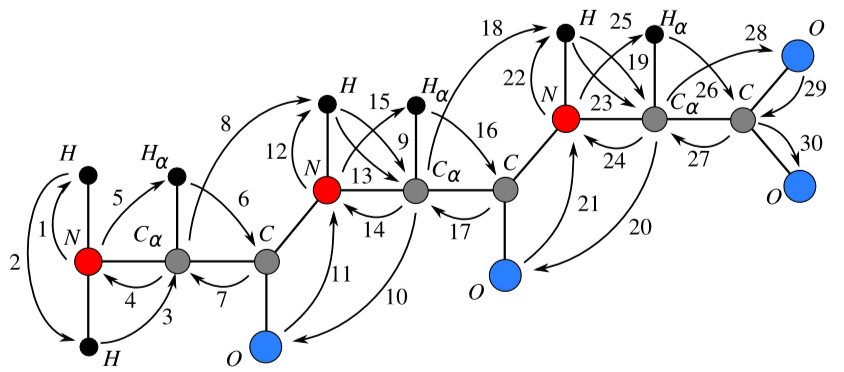
\includegraphics[width=0.8\linewidth]{hcVO.png}
		\end{center}
		\caption{Esboço da ordenação HC \cite{carlile:MinimalOrder}.}
		\label{fig:hcVO}
	\end{figure}	
	Define-se a ordem HC como:
	
	\begin{minipage}{0.532\linewidth}
		$$
		hc = \{ N^1, H^1, H^{1'}, C_{\alpha}^1, N^1, H_{\alpha}^1, C^1, C_{\alpha}^1, \dots,
		$$
		
	\end{minipage}
	%\vspace{-0.1cm}
	$$
	H^i, C_{\alpha}^i, O^{i-1}, N^i, H^i, C^{i}_\alpha, N^i, H^{i}_\alpha, C^i, C_{\alpha}^i,\dots,
	$$
	
	\hspace{4.5cm}
	\begin{minipage}{0.532\linewidth}
		\vspace{-0.7cm}
		$$
		H^p, C_{\alpha}^p, O^{p-1}, N^p, H^p, C^{p}_\alpha, N^p, H^{p}_\alpha, C^p, C_{\alpha}^p, O^p, C^p, O^{p'}\}
		$$
	\end{minipage}
	\\

	Onde, como na Figura ~\ref{fig:hcVO}, $i = 2, \dots, p-1$, $H^{1'}$ é o segundo hidrogênio ligado ao $N^1$ e $O^{p'}$ é o segundo oxigênio ligado ao $C^p$.
	
	Dado nossas hipóteses do problema, fica trivial perceber que essa ordenação respeita as condições (a) e (b), a menos de duas informações que podem não ser tão óbvias. Primeiramente: Toda distância entre hidrogênios relativamente próximos --- inclusive entre $H_\alpha^{i-1}$ e $H^{i}$ --- são dados pela RMN. A segunda informação pertinente é que, para respeitar a condição (a) no átomo $H^i$, precisamos ter conhecimento do plano mostrado na Figura ~\ref{fig:peptidica}, que diz que os átomos em torno da ligação peptídica são coplanares --- e, por tanto, pode-se descobrir a distância entre o $H^i$ e $C_\alpha^{i-1}$ através das leis de senos e cossenos. 
 	
 	Nesse momento, é importante mencionar que o software PDBReader implementa a ordenação HC (como pode ser visto no componente 6 da Figura ~\ref{fig:pdbreader}), ou seja, este trabalho também tem como resultado final uma automação do processo de criação de instâncias de proteínas ordenadas a partir de dados de moléculas reais vindas do wwPDB. Vale mencionar que essa é uma ferramenta valiosa do ponto de vista acadêmico, uma vez que possibilita a entrada de dados reais para testes --- é comum, na literatura, a utilização de instâncias artificiais nos testes \cite{carlile:BP} \cite{carlile:instancesMDGP}.
 	
 	A ordenação HC gera uma estrutura muitíssimo interessante para se trabalhar. De fato, por garantir que sempre tenhamos pelo menos um 3-click em todo átomo com posto maior que três, podemos tentar encontrar a realização do próximo átomo da sequência $v_i$ com $i \geq 4$, utilizando a interseção das 3 esferas centradas nos três átomos anteriores $v_{i-3}, v_{i-2}$ e $v_{i-1}$ (já realizados) e com os respectivos raios iguais as distâncias $d_{i,i-3}, d_{i,i-2}$ e $d_{i,i-1}$ para o átomo $i$ que se está tentando localizar. 
 	
 	Essas intersecções tem três possibilidades associadas (veja Figura ~\ref{fig:esferas}): Ou não temos nenhum ponto de interseção entre elas --- e isso não acontece, pois fere as hipóteses do problema, logo, só ocorre se existe alguma informação incorreta; Ou existe um ponto --- donde os átomos são colineares e isso também nunca acontece, devido aos ângulos típicos das ligações; ou existem dois pontos onde as esferas se interceptam --- este é o caso geral.
 	
 	\begin{figure}[H]
 		\begin{center}
 			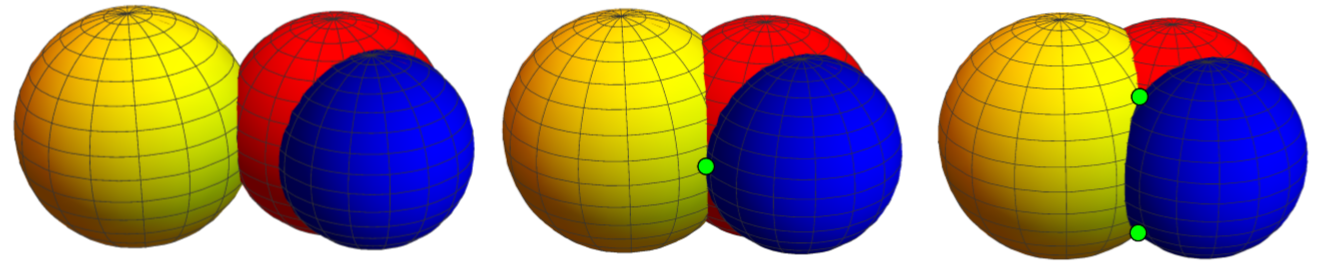
\includegraphics[width=0.8\linewidth]{esferas.png}
 		\end{center}
 		\caption{Interseção de três esferas \cite{carlileBook31Coloquio}.}
 		\label{fig:esferas}
 	\end{figure}
 	
 	Perceba, então, que além da ordenação dos vértices garantir a finitude do conjunto solução do problema, ela também organizar o espaço onde devemos fazer a busca por uma solução. Na verdade, a ordem induz uma estrutura de \textit{árvore binária} no espaço de busca \cite{fidalgotese}. De fato, conforme discussão anterior entorno da Equação ~\ref{eq:cosOmega}, sempre temos duas possibilidades para posicionar o próximo átomo da molécula \cite{carlileGDandAplications} --- pois, como já dito, possuímos dois $\mbox{sen}(\omega_{ijkl})$ associados, um positivo e outro negativo. Com isso, ganhamos uma discretização do problema (pois saímos espaço contínuo de soluções), nos permitindo definir uma nova variante para ele.
 	
 	\subsection{\textit{Discretizable Molecular Distance Geometry Problem}}
 	Esse é o problema central desse texto. Trata-se do MDGP monido de uma ordenação conveniente que permite sua discretização, como segue formalmente definido.
 	
 	\begin{center}
 		\begin{minipage}{0.9 \linewidth}
 			\textbf{\textit{Discretizable Molecular Distance Geometry Problem:}} Dados um grafo ponderado e não-direcionado $G = (V,E,d)$ associado a um MDGP, onde $d: E \longrightarrow \mathbb{R}_{+}$, o subconjunto de vértices iniciais $U_{0} = \{v_{1},v_{2},v_{3} \}$ e uma relação de ordem total em $V$ que satisfaça a seguinte relação de axiomas:
 			\begin{enumerate}
 				\vspace{-0.2cm}
 				\item $G[U_{0}]$ é um clique em três vértices (iniciando a configuração);
 				\vspace{-0.2cm}
 				\item para todo vértice $v_{i}$ com posto $i = \rho(v_{i}) > 3$ nesta ordem, $G[U_{i}]$ é uma clique com quatro vértices (ordem de discretização, dada anteriormente) e
 				\vspace{-0.2cm}
 				\item para cada vértice $v_{i}$, com posto $i = \rho(v_{i}) > 3$, juntamente com $\{ v_{i-3}, v_{i-2} , v_{i-1} \}$, vale a desigualdade
 				\vspace{-0.25cm}
 				\begin{center}
 					$d_{i-3,i-1} < d_{i-3,i-2} + d_{i-2,i-1},$ \hspace{0.5cm} (Desigualdade Triangular Estrita)
 				\end{center}
 			\end{enumerate}
 			\vspace{-0.2cm}
 			\underline{encontre uma imersão} $x: V \longrightarrow \mathbb{R}^{3}$ tal que valha $\left\| x(v_{i}) - x(v_{j}) \right\| = d_{i,j}$, $\forall \{v_{i},v_{j} \} \in E$.
 		\end{minipage}
 	\end{center}
 	
 	Note que, usando os valores de distâncias das cliques $\{ v_{i-3}, v_{i-2} , v_{i-1}, v_i \}$, temos gratuitamente todas as distâncias entre átomos consecutivos $d_{1,2}, \dots, d_{n-1, n}$, além de podermos obter facilmente os ângulos planos $\theta_{1,3}, \dots, \theta_{n-2, n}$ usando a Lei dos Cossenos (vide Apêndice A).
 	
 	Lembrando que só precisamos das coordenadas internas para definir a estrutura 3D das proteínas --- visto que podemos aplicar o conjunto de matrizes $B_i$ para realizar a conversão dos sistemas de coordenadas. Como temos todas as distâncias e ângulos planos, só nos falta verificar os ângulos de torção $\omega_{1,4}, \dots, \omega_{n-3, n}$, que, como vimos, sempre possuímos dois ($\omega_{i-3, i}^1$ e $\omega_{i-3,i}^2$) possíveis ângulos associados. Essa estrutura binária de decisão é ilustrado na Figura ~\ref{fig:torcao}, onde temos as duas posições possíveis ($i$ e $i^\prime$) para o último vértice.
 	
 	\begin{figure}[H]
 		\begin{center}
 			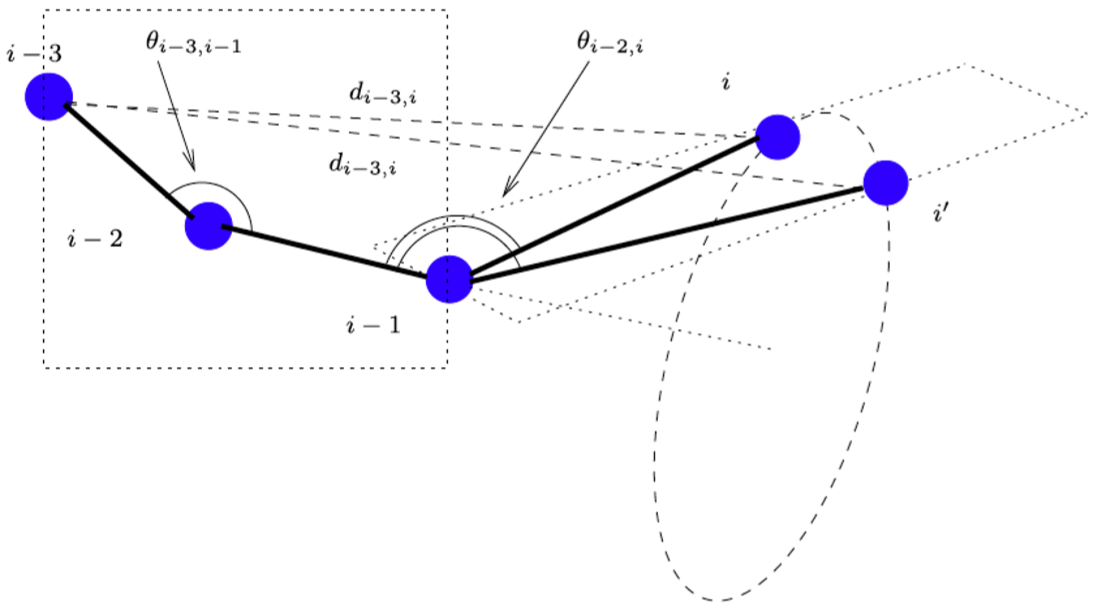
\includegraphics[width=0.85\linewidth]{torcao.png}
 		\end{center}
 		\caption{Duas possibilidades para o ângulo de torção \cite{carlile:DMDGP}.}
 		\label{fig:torcao}
 	\end{figure}
 	
 	Uma das conclusões mais interessantes que partem dessa análise é que não precisamos mais resolver os sistemas quadráticos que definem o DGP, problema fundamental de Geometria de Distâncias --- que antes envolviam otimização contínua, complicada do ponto de vista computacional, com a quantidade de mínimos locais explodindo para moléculas demasiadamente grandes ---, pois já temos definidas as posições possíveis para cada vértice. Logo, nosso problema se restringiu apenas a decidir quais são os ângulos de torção corretos.
 	
	\newpage
	\section{\textit{Branch-and-Prune}}
	 Introduzimos o capítulo anterior com a definição do problema fundamental da nossa área, o \textit{Distance Geometry Problem}, que não tardou ao ceder seu lugar de destaque para o \textit{Molecular Distance Geometry Problem} --- sendo exatamente o mesmo problema, porém, com o espaço fixado em $\mathbb{R}^3$. Em seguida fomos apresentados ao \textit{Discretization Vertex Order Problem}, que, de posse de uma de suas soluções, nos permitiu construir uma versão discreta do nosso problema, chegando, finalmente, no \textit{Discretizable Molecular Distance Geometry Problem} --- que se trata do MDGP monido de uma ordem esperta para seus vértices.
	
	As vezes parece que o universo conspira a favor da beleza de uma solução matemática. A ordenação nos átomos da molécula, além de reduzir infinitamente o conjunto solução do problema \cite{carlileBook31Coloquio}, ainda induziu uma estrutura de \textbf{árvore binária} para os pontos que sobraram \cite{fidalgotese}, que logo deu origem a um algorítimo que se aproveita dessa estrutura para reduzir ainda mais o conjunto solução do problema --- o algorítimo Branch-and-Prune, tema desse capítulo. E mais: por conta dessa estrutura, ficou fácil perceber --- visualmente mesmo --- que existe uma simetria intrínseca nas diferentes soluções do DMDGP (que normalmente não tem solução única, devido as várias conformações moleculares). De fato, parece que o universo conspirou a favor desta solução. É belíssima.
	
	\subsection{O Algorítimo}
	Apresentado em 2007 \cite{carlile:BP}, por Leo Liberti, Carlile Lavor e Nelson Maculan, este algorítimo (também chamado BP, com grande similaridade ao Branch-and-Bound) consiste em uma estratégia numérica recursiva, que resolve o DMDGP eficientemente utilizando uma busca combinatória no espaço de busca de soluções, onde realiza-se vértice por vértice do sistema, seguindo a ordem dada, ``podando'' --- isto é, descartando --- todo sub-conjunto solução do sistema que não esteja de acordo com as informações pré-estabelecidas. Desde que ele foi publicado, tem se verificado tanto sua beleza matemática, quanto a sua eficiência numérica-computacional para resolver problemas em Geometria de Distâncias.
	
	Como todo algorítimo, esse possui um conjunto de entradas e saídas.
	\begin{description}
		\item[Entradas:] O grafo $G(V, E, d)$ que define o DMDGP --- onde possuímos uma ordenação para $V$ --- e mais um escalar $\varepsilon \in \mathbb{R}$ que da a tolerância aceita no algoritmo (pois o BP não é um método exato, encontrando apenas soluções distantes a menos de $\varepsilon$ das reais).
		
		Para facilitar a utilização do algorítimo, também faremos uma distinção dos vértices que compõem o conjunto $E$: Sejam os subconjuntos $E_{d}, E_p \subset E$, tal que $E = E_{d} \cup E_{p}$ --- denominados como, respectivamente, \textit{arestas de discretização} e \textit{arestas de poda} ---, onde
		
		\begin{center}
			$E_{d} = \{\{v_i,v_j\} \in E : |i-j|\leq 3\}$ e $E_{p} = E - E_d$.
		\end{center}
		
		\item[Saídas:] Uma árvore binária $T$, onde cada nó de nível $i$ da árvore é uma realização possível do vértice $v_i \in V$, de tal forma que o caminho $C \subset T$ partindo da raiz (primeiro nó) até uma folha de nível $n = |V|$ da árvore seja uma solução para o problema, isto é, um conjunto de realizações de todos os átomos da molécula.
	\end{description}

	São três fases que definem o algoritmo: Inicialização, \textit{Branching} e \textit{Pruning} \cite{fidalgotese}.
		
	\subsubsection*{Inicialização}
	Esta etapa se preocupa com a inicialização da estrutura. Ela define a realização dos três primeiros átomos $v_1, v_2$ e $v_3 \in V$ da sequência, que são posicionados nas respectivas posições $x_1, x_2$ e $x_3 \in \mathbb{R}^3$, utilizando as operações contidas nas matrizes $B_1, B_2$ e $B_3$ (ver Capitulo ~\ref{sec:bi}). Obtendo os pontos 	
	$$
	x_1\:=\:
	\begin{bmatrix}
	0\\ 
	0\\  
	0
	\end{bmatrix},\:\:\:
	x_2\:=\:
	\begin{bmatrix}
	-d_{1,2}\\ 
	0\\  
	0
	\end{bmatrix},\:\:\:
	x_3\:=\:
	\begin{bmatrix}
	-d_{1,2}+d_{2,3}\cos\theta_{1,3}\\ 
	d_{2,3}\mbox{sen}\theta_{1,3}\\  
	0
	\end{bmatrix}.
	$$
	
	Essas três primeiras posições estão associados biunivocamente com os três primeiros nós da arvore de busca $T$ (representada por um grafo), que também é iniciada, conforme Figura ~\ref{fig:bp1}
	
	\begin{figure}[H]
		\begin{center}
			
\includegraphics[width=0.035\linewidth]{bp1.png}
		\end{center}
		\caption{Inicialização de T \cite{fidalgotese}.}
		\label{fig:bp1}
	\end{figure}
		
	\subsubsection*{\textit{Branching}}
	Essa etapa está associada com o processo de ``ramificação'' de $T$ \cite{fidalgotese}. Ou seja, supondo que já foram realizados os vértices $v_1, \dots, v_{i-1}$ (onde $3 < i< |V|$), repeitando a ordenação em $V$, nosso objetivo é obter a realização $x_i = (x_{i1}, x_{i2}, x_{i3}) \in \mathbb{R}^3$ do vértice $v_i \in V$.
	
	Para isso, basta calcularmos o produto matricial mostrado no Capitulo ~\ref{sec:bi}:
	
	$$
	\begin{bmatrix}
	x_{i1}\\ 
	x_{i2}\\ 
	x_{i3}\\ 
	1
	\end{bmatrix}
	= C_{i}\begin{bmatrix}
	0\\ 
	0\\ 
	0\\ 
	1
	\end{bmatrix},
	$$
	onde $C_i = C_{i-1}B_i = \prod_{j=1}^{i}B_j$ é dita o \textit{produto acumulado} das matrizes de torção $B_j$, que, para $j>3$, são dadas por
	
	$$\hspace{-1.1cm}
	B_{j}=\begin{bmatrix}
	-\cos(\theta_{j-2,j}) & -\mbox{sen}(\theta_{j-2,j}) & 0 & -d_{j-1,j}\cos(\theta_{j-2,j}) \\
	\mbox{sen}(\theta_{j-2,j})\cos(\omega_{j-3,j}) & -\cos(\theta_{j-2,j})\cos(\omega_{j-3,j}) & -\mbox{sen}(\omega_{j-3,j}) & d_{j-1,j}\hspace{0.1cm}\mbox{sen}(\theta_{j-2,j})\cos(\omega_{j-3,j}) \\
	\mbox{sen}(\theta_{j-2,j})\hspace{0.1cm}\mbox{sen}(\omega_{j-3,j}) & -\cos(\theta_{j-2,j})\hspace{0.1cm}\mbox{sen}(\omega_{j-3,j}) & \cos(\omega_{j-3,j}) & d_{j-1,j}\hspace{0.1cm}\mbox{sen}(\theta_{j-2,j})\hspace{0.1cm}\mbox{sen}(\omega_{j-3,j}) \\
	0 & 0 & 0 & 1
	\end{bmatrix}.
	$$
	
	Porém, como $\mbox{sen}(\omega_{j-3,j}) = \pm\sqrt{1 - \cos(\omega_{j-3,j})^2}$, sempre temos duas matrizes de torção $B_j^1$ e $B_j^2$ associadas a cada vértice $v_j$. É a este fato que está associado o conceito de ramificação, pois, a cada matriz de torção temos como resultado um novo conjunto de realizações, que se visualiza como um novo ramo de $T$. 
	
	Ilustramos esse processo na Figura ~\ref{fig:ramificacoes}, que presume um DMDGP com $|V| = 6$. Ou seja, obtemos $2^{6-3} = 2^3 = 8$ possíveis soluções, dadas pelas suas três ramificações.
	
	\begin{figure}[H]
		\begin{center}
			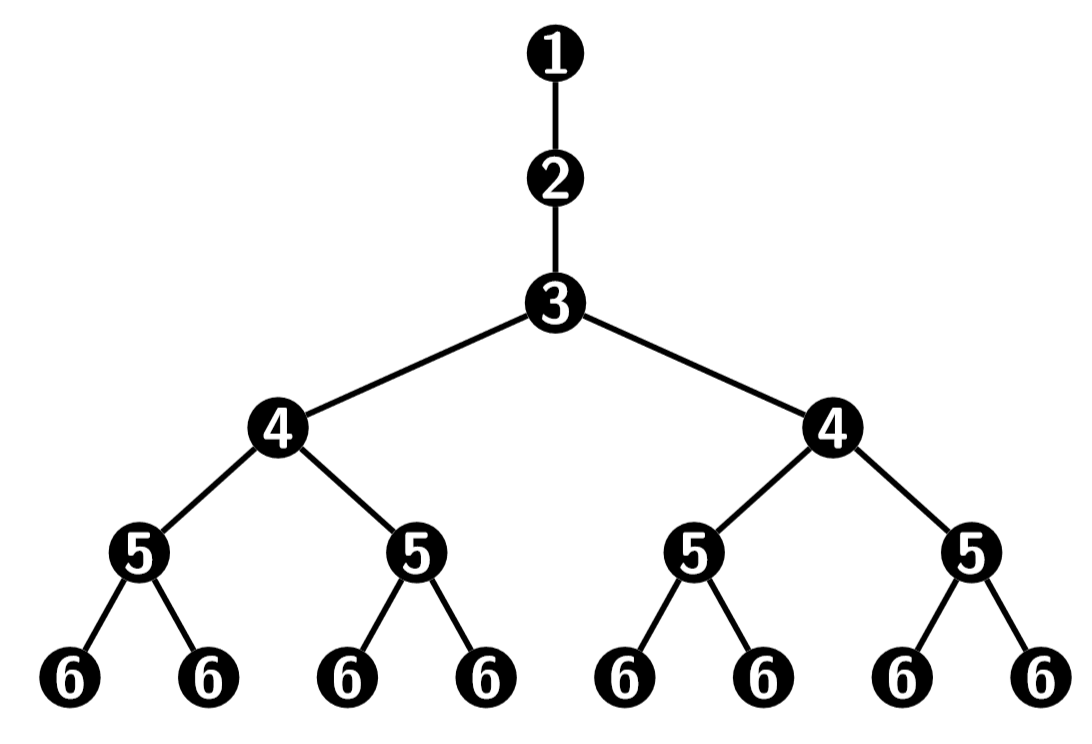
\includegraphics[width=0.45\linewidth]{ramificacoes.png}
		\end{center}
		\caption{Árvore $T$ completa de uma instância DMDGP com 6 vértices \cite{fidalgotese}.}
		\label{fig:ramificacoes}
	\end{figure}
	
	Fica claro aqui que o processo de ramificação garante que, no máximo, existem $2^{n-3}$ soluções possíveis para o problema. Isso colabora com a enumerabilidade e finitude do conjunto solução do problema, porém, também mostra que o número de soluções cresce de uma forma exponencial com o crescimento da molécula.
	
	\subsubsection*{\textit{Pruning}}
	Essa etapa tem como função diminuir drasticamente o conjunto solução do problema. Conseguimos isso ao classificar os diferentes ramos de $T$ (gerados pelos diferentes ângulos de torção $\omega_{i-3,i}^1$ e $\omega_{i-3,i}^2$) como factíveis ou não e, então, ``podando'' os infactíveis.  
	
	Como já discutimos antes, para calcular as matrizes de torção da etapa anterior só precisamos dos dados do 3-clique garantido pelas hipóteses do DMDGP, ou seja, das distâncias $d_{i,i-3}, d_{i,i-2}$ e $d_{i,i-1}$ associadas aos elementos de $E_d$. Com isso, todas as distâncias associados aos elementos de $E_p$ podem ser consideradas como dados adicionais para o problema. 
	
	Perceba que, para todo $v_j$ tal que $\{v_i,v_j\} \in E_p$, se conhecemos a realização de $v_j$, a distância extra $d_{i,j}$ pode ser enxergada, do ponto de vista geométrico, como uma esfera extra àquelas outras três dadas pelo 3-clique. Isso gera a interseção de quatro esferas no $\mathbb{R}^3$, donde podemos ter apenas uma das duas possibilidades: Ou elas se interceptam em um único ponto (veja Figura ~\ref{fig:quatroesferas}) ou em nenhum. 

	\begin{figure}[H]
		\begin{center}
			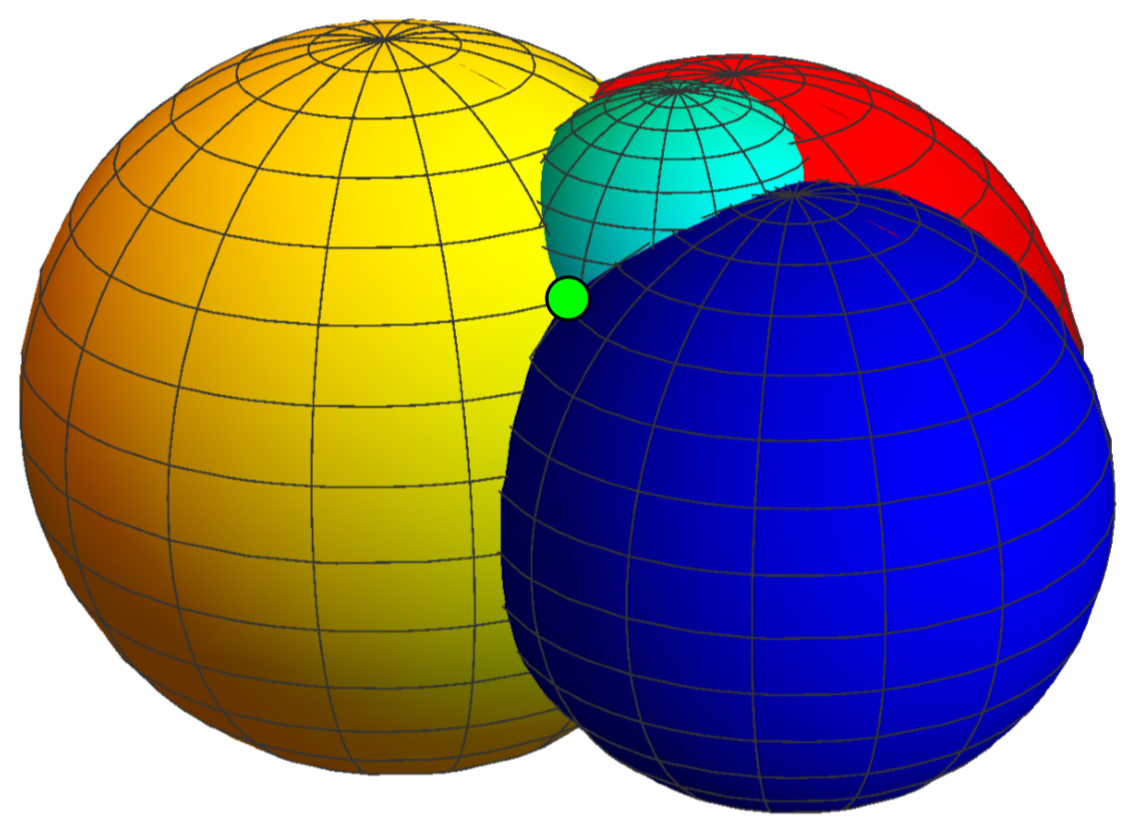
\includegraphics[width=0.35\linewidth]{quatroesferas.png}
		\end{center}
		\caption{Interseção de quatro esferas no $\mathbb{R}^3$ \cite{carlileBook31Coloquio}.}
		\label{fig:quatroesferas}
	\end{figure}
	
	E é este o princípio da factibilidade de um ramo: Sempre que estamos na etapa de \textit{Branching} --- ou seja, calculando uma realização $x_i$ de $v_i$ a partir de uma matriz de torção ---, podemos verificar se existe uma distância extra, associada a algum elemento $\{v_i,v_j\} \in E_p$ tal que $j < i$ e, caso exista, podemos verificar se $|x_i - x_j| < \varepsilon$. Caso for, significa que o ramo é factível e, caso não for, podemos descartar (``podar'') todas as soluções associadas a sub-árvore definida por aquele ramo.
	
	A etapa de \textit{pruning} é ilustrada na Figura ~\ref{fig:poda} (adaptada de \cite{fidalgotese}). Dando continuidade ao exemplo da Figura ~\ref{fig:ramificacoes}, agora temos $E_p = \{\{v_1,v_5\},\{v_2,v_6\}\}$, o que nos permitiu testar a factibilidade dos ramos associados ao $v_5$ e ao $v_6$ e podar os infactíveis, diminuindo consideravelmente o conjunto solução.
	
	\begin{figure}[H]
		\begin{center}
			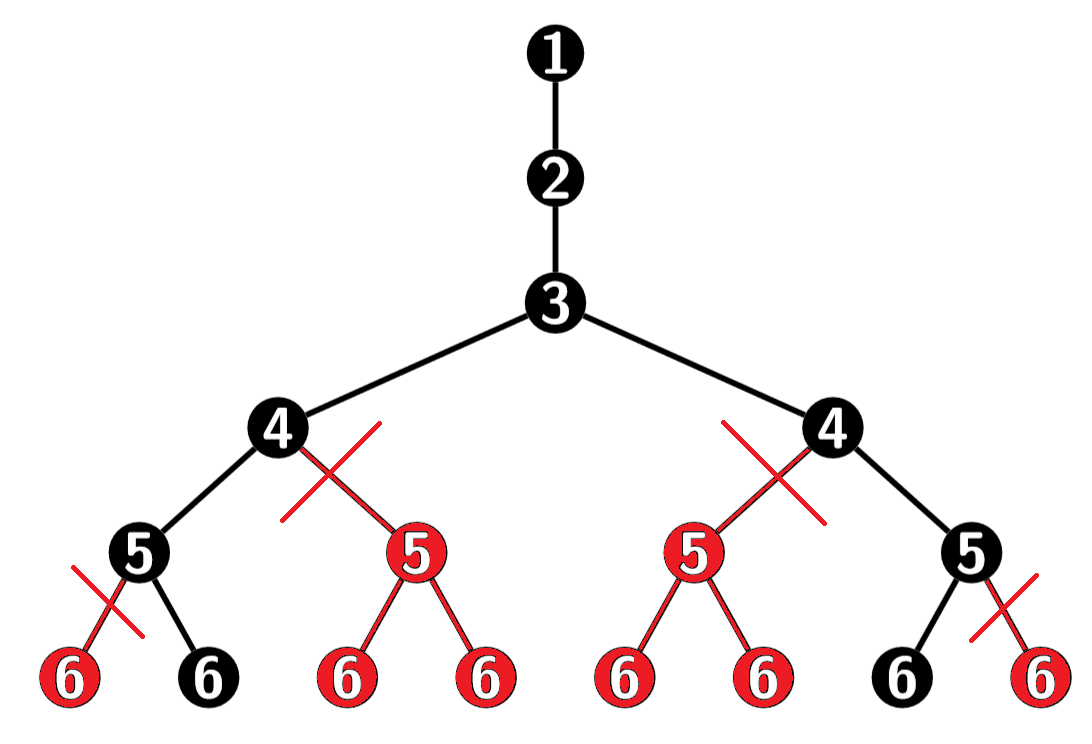
\includegraphics[width=0.45\linewidth]{prune.png}
		\end{center}
		\caption{Árvore $T$ de um DMDGP de 6 vértices com a poda evidenciada.}
		\label{fig:poda}
	\end{figure}

	Perceba que o crescimento exponencial de soluções ($2^{n-3}$) da etapa de \textit{branching} está associado com o DMDGP ser um problema NP-Difícil. Por conta disso é que esse algorítimo tem tanta beleza associada, isto é, apesar da grande complexidade de se resolver o problema original, o BP pode encontrar rapidamente essas soluções.

	Mas uma dúvida ainda é importante: O conjunto $E_p = \emptyset$? Neste caso, $E = E_d$ e, portanto, todas as posições finais são factíveis trivialmente. Dessa forma, todas as $2^{n-3}$ realizações encontradas durante a etapa de \textit{branching} representam soluções possíveis para o DMDGP, o que, é claro, é o nosso pior caso, pois o BP precisa continuar a exploração de todos os $2^{n-3}$ nós de $T$. 
	
	Por outro lado, se utilizarmos a ordenação hc apresentada no Capitulo ~\ref{sec:hc} como ordem que define o DMDGP, nós garantimos que $E_p \neq \emptyset$. Essa é uma das vantagens dessa ordenação. Na verdade, muito mais do que não vazio, graças as propriedades geométricas das proteínas estudadas em \cite{carlile:MinimalOrder} nós podemos enunciar o seguinte resultado (extraído de \cite{carlile:MinimalOrder}): 

	\textbf{Teorema:} Usando a ordenação hc, considerando que todos os ângulos e distâncias das ligações atômica estão fixadas nos seus valores de equilíbrio energético (essa é conhecida como \textit{hipótese de geometria rígida}), que os átomos ao redor das ligações peptídicas formam um plano, que as posições possíveis para $C_\alpha^1$ e $C^j$ (com $j = 1, \dots,p$) são únicas --- devido a propriedade quiral do tetraedro formado por $\{N^1, H^1, H^{1\prime}, C_\alpha^1\}$ e $\{C_\alpha^j, N^j, H^j_\alpha,C^j\}$ --- e, dado o conjunto de distâncias entre os pares de átomos de hidrogênio
	
	$$\{H^{1\prime}, H^1_\alpha\}, \dots, \{H_\alpha^{i-1}, H^i\}, \{H^i, H^i_\alpha\}, \{H^i_\alpha, H^{i+1}\}, \dots, \{H^p, H^p_\alpha\}$$
	(onde $i = 2, \dots, p-1$ e $p$ é o número de aminoácidos que compõem a proteína), as ramificações na árvore de busca só ocorrem em átomos de hidrogênio dados por
	$$\{H_\alpha^1, \dots, H^i, H_\alpha^i, \dots, H^p, H_\alpha^p\}.$$	
	
	\subsection{Estrutura Algorítmica}
	Agora que a ideia por trás do BP está desenvolvida nos três passos anteriores (inicialização, \textit{branching} e \textit{pruning}) podemos apresenta-lo formalmente como um algorítimo de uma função recursiva, como segue.
	\\
	
	\begin{algorithm}[H]
		BranchAndPrune($T,v,i$)\\
		\uIf{$i\leq n-1$}{
			Calcule as matrizes de torção $B_i^1$ e $B_i^2$;\\
			Recupere a matriz de torção acumulada $C_{i-1}$ referente ao nó-pai $P(v)$;\\
			Calcule as próximas matrizes de torção acumuladas $C_i = C_{i-1}B_i^1$ e $C_i^\prime=C_{i-1}B_i^2$;\\
			Utilize-as para calcular as posições $x_i = C_iy$ e $x_i^\prime = C_i^\prime y$;\\
			Seja $\lambda = 1, \rho = 1$;\\
			\ForEach{$\{v_j,v_i\} \in E_p$ com $j<i$}{
				\If{$(||x_j - x_i||^2 - d_{ij}^2)^2 > \varepsilon$}{
					$\lambda = 0$;	
				}	
				\If{$(||x_j - x_i^\prime||^2 - d_{ij}^2)^2 > \varepsilon$}{
					$\rho = 0$;	
				}	
			}
			
			\uIf{$\lambda = 1$}{
				Crie um nó $z$, armazenando $C_i$ e $x_i$ e fazendo $P(z) = v$ e $L(v) = z$;\\
				Faça $T \leftarrow T \cup \{z\}$;\\
				BranchAndPrune($T,z,i+1$);
			}\Else{
				Faça $L(v) =$ PRUNED;
			}
			\uIf{$\rho = 1$}{
				Crie um nó $z^\prime$, armazenando $C_i^\prime$ e $x_i^\prime$ e fazendo $P(z^\prime) = v$ e $R(v) = z^\prime$;\\
				Faça $T \leftarrow T \cup \{z^\prime\}$;\\
				BranchAndPrune($T,z^\prime,i+1$);
			}\Else{
				Faça $R(v) =$ PRUNED;			
			}	
		}
		\Else{
			Solução está armazenada nos nós-pais de $n$ a $1$, em busca retrocedida.
		}
		\caption{Algoritmo BP \cite{fidalgotese} \cite{carlile:BP}}
	\end{algorithm}
	
	\subsection{Simulações Computacionais}
	Lorem ipsum es bons para fodis a tchuca cakopsa apsokdpaksdpak apskdam gn an foamcorhba asidj dpao kafhrauh a jdoaiho ao naob eubf aohua asd.
	
	
	\newpage
	\section{Considerações Finais}
	
	\newpage
	\phantomsection
	\addcontentsline{toc}{section}{Referências}
	
	\bibliographystyle{unsrt}
	\bibliography{references}
	
	% ======================================================================================================================================================================================================%
	
	\newpage
	\phantomsection
	\addcontentsline{toc}{section}{Apêndice A - Lei dos Cossenos e Ângulos Entre dois Vetores no $\mathbb{R}^3$}
	
	\section*{Apêndice A}
	\subsection*{Lei dos Cossenos e Ângulos Entre dois Vetores no $\mathbb{R}^3$}
	
	\subsubsection*{Leis dos Cossenos}

	A lei dos cossenos é uma propriedade trigonométrica válida para qualquer triângulo, permitindo encontrar o valor de um dos seus lados conhecendo apenas os outros lados e um ângulo. Porém, aqui utilizaremos a ideia reversa, onde, nesse caso, saberemos os lados e queremos descobrir os ângulos.
		\begin{figure}[H]
		\begin{center}
			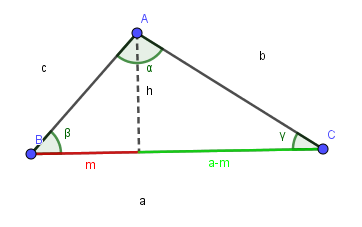
\includegraphics[width=0.50\linewidth]{triangulo.png}
		\end{center}
		\caption{Triângulo para ilustrar a lei dos cossenos.}
		\label{fig:coslaw}
	\end{figure}
	\begin{itemize}
		\item \textbf{Demonstração Leis dos Cossenos:}
		
		Dado um triângulo qualquer, traça-se uma altura relativa ao lado $a$. Aplicando o \textit{Teorema de Pitágoras} no $\Delta ABD$:
		
		\begin{equation}
		c^{2}=m^{2}+h^{2} \rightarrow h^{2}=c^{2}-m^{2}
		\label{eq:tri1}
		\end{equation}
		
		Aplicando novamente \textit{Pitágoras}, porém, em $\Delta ADC$, obtemos:
		\begin{equation}
		b^{2}=h^{2}+(a-m)^{2}
		\label{eq:tri2}
		\end{equation}
		Substituindo na equação ~\ref{eq:tri2} o valor de $h^{2}$ obtido em ~\ref{eq:tri1}:
		$$
		b^{2}=c^{2}-m^{2}+a^{2}-2am+m^{2}
		$$
		$$
		b^{2}=c^{2}+a^{2}-2am
		$$
		Analisando a 
		Figura ~\ref{fig:coslaw}, pode-se perceber que $\frac{m}{c}=\cos\beta$, então:
		$$
		b^{2}=c^{2}+a^{2}-2ac\cos\beta
		$$
		Analogamente, obtém-se:
		$$
		c^{2}=a^{2}+b^{2}-2ab\cos\gamma
		$$
		$$
		a^{2}=b^{2}+c^{2}-2bc\cos\alpha
		$$
		Note também que se o argumento dos cossenos for $\frac{\pi}{2}$ recaímos no Teorema de Pitágoras. $\hfill\blacksquare$
		\item \textbf{Ângulos Entre 2 Vetores:}
		
		Sejam dois vetores $\overrightarrow{u}$ e $\overrightarrow{v} \in \mathbb{R}^2$, representados na Figura ~\ref{fig:diffbtvet}
		\begin{figure}[H]
			\begin{center}
				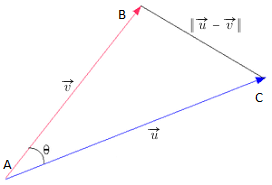
\includegraphics[width=0.4\linewidth]{Angulovetoresnovo.png}
			\end{center}
			\caption{Diferença entre vetores u e v}
			\label{fig:diffbtvet}
		\end{figure}
		Para encontrarmos o angulo $\theta$ utilizaremos a lei dos cossenos aplicada a $\Delta ABC$:
		\begin{equation}
		\|\overrightarrow{u}-\overrightarrow{v}\|^{2}=\|\overrightarrow{u}\|^{2} + \|\overrightarrow{v}\|^{2} - 2\|\overrightarrow{u}\|\|\overrightarrow{v}\|\cos\theta
		\label{eq:ang1}
		\end{equation}
		Utilizando a definição do produto escalar \cite{GASteinbruch}
		\begin{equation}
		\|\overrightarrow{u}-\overrightarrow{v}\|^{2}=\|\overrightarrow{u}\|^{2} + \|\overrightarrow{v}\|^{2} - 2\overrightarrow{u}\overrightarrow{v}
		\label{eq:ang2}
		\end{equation}
		Comparando a equação ~\ref{eq:ang1} com a ~\ref{eq:ang2}, obtemos trivialmente
		$$
		\|\overrightarrow{u}\|^{2} + \|\overrightarrow{v}\|^{2} - 2\|\overrightarrow{u}\|\|\overrightarrow{v}\|\cos\theta = \|\overrightarrow{u}\|^{2} + \|\overrightarrow{v}\|^{2} - 2\overrightarrow{u}\overrightarrow{v}
		$$
		$$
		\overrightarrow{u}\overrightarrow{v} = \|\overrightarrow{u}\|\|\overrightarrow{v}\|\cos\theta
		$$
		Logo,
		$$
		\cos\theta = \frac{\overrightarrow{u}\overrightarrow{v}}{\|\overrightarrow{u}\|\|\overrightarrow{v}\|} 
		$$
		$\hfill\blacksquare$
	\end{itemize}
	
	\newpage
	\phantomsection
	\addcontentsline{toc}{section}{Apêndice B - Matrizes como Transformações Lineares e Sobre $B_i$}
	\section*{Apêndice B} 
	\subsection*{Matrizes como Transformações Lineares e Sobre $B_i$}
	
	Quando se começa a aprender sobre matrizes, no ensino médio, normalmente este é um assunto que lhe é apresentado como algo que caiu do céu, difícil de engolir. Na verdade, não é raro um graduando de matemática ter dificuldades para entende-las.
	
	\subsubsection*{Matrizes}
	
	Uma matriz real $\mathbf{a} = [a_{ij}]$ de dimensões $m \times n$ é definida como uma lista de números $a_{ij}$, onde $i \mid 1 < i < m$ e $j \mid 1 < j < n$ são os índices que, juntos, identificam unicamente cada elemento. Costuma-se representar a matriz $\mathbf{a}$ como um quadro de $m\cdot n$ elementos, onde $m$ é o número de linhas e $n$ é o número de colunas, de forma que o elemento $a_{ij}$ situa-se no cruzamento entre a $i$-ésima linha e a $j$-ésima coluna, como segue:
	
	\[ \mathbf{a} =
	\begin{blockarray}{cccc}
	\begin{block}{[cccc]}
	a_{11} & a_{12} & \cdots & a_{1n} \\
	a_{21} & a_{22} & \cdots & a_{2n} \\
	\vdots & \vdots & \vdots & \vdots \\
	a_{m1} & a_{m2} & \cdots & a_{mn} \\
	\end{block}
	\end{blockarray}\]
	
	Seja $M(m\times n)$ um conjunto de matrizes de tal forma que todas as matrizes de dimensão $m\times n$ estejam dentro dele. Podemos definir algumas operações neste conjunto. São elas: 
	
	\begin{itemize}
		\item \textbf{Soma de Matrizes:} Sejam duas matrizes $\mathbf{a}, \mathbf{b}$ $\in M(m \times n)$, define-se a soma de $\mathbf{a} = [a_{ij}]$ com $\mathbf{b} = [b_{ij}]$ como $$\mathbf{a} + \mathbf{b} = [a_{ij} + b_{ij}]$$
		
		\item \textbf{Multiplicação por Escalar:} Sejam $\mathbf{a} \in M(m \times n)$ e $\lambda \in \mathbb{R}$ um escalar qualquer, o produto de $\mathbf{a} = [a_{ij}]$ por $\lambda$ é definido como $$\lambda \cdot \mathbf{a} = \lambda [a_{ij}] = [\lambda a_{ij}]$$
	\end{itemize}
	
	Tendo estas duas operações construídas, podemos definir também:
	\begin{itemize}
		\item \textbf{Existência de elemento nulo:} Define-se como \textit{matriz nula} $\mathbf{0} \in M(m \times n)$ a matriz formada exclusivamente por $m\cdot n$ zeros.
		
		\item \textbf{Existência do elemento oposto para adição:} Seja $\mathbf{a} \in M(m \times n)$ uma matriz da forma $\mathbf{a} = [a_{ij}]$, define-se o elemento oposto de $\mathbf{a}$ como $-\mathbf{a} = [-a_{ij}].$
	\end{itemize}

	Tendo tais definições, chegamos em um resultado interessante.
	\\
	
	\textbf{Proposição: }O conjunto $M(m \times n)$ é um espaço vetorial. \cite{AlgebraLinearElon}
	\\ \newline	Para chegar na conclusão acima, basta tomar as definições dadas e perceber que podemos escrever cada linha e coluna de uma matriz como vetores, ou seja, $\forall \mathbf{a} \in M(m \times n)$, $\exists$ um \textit{vetor-linha} $a_i^l = (a_{i1}, a_{i2}, \dots, a_{in})$ e um \textit{vetor-coluna} $a_j^c = (a_{1j}, a_{2j}, \dots, a_{mj})$ que representam a $i$-ésima linha e $j$-ésima coluna de $\mathbf{a}$, respectivamente.
	
	Para que possamos continuar, necessitamos introduzir mais um grande tópico de álgebra linear, as \textit{transformações lineares}.
	\subsubsection*{Transformações Lineares}
	Sejam $E, F$ espaços vetoriais. Uma transformação linear $A: E \longrightarrow F$ é uma correspondência que associa a cada vetor $v \in E$ um vetor $A(v) = A\cdot v = Av \in F$ de modo que valham, para quaisquer $u,v \in E$ e $\alpha \in \mathbb{R}$, as relações:  
	$$A(u + v) = A(u) + A(v),$$
	$$A(\alpha\cdot v) = \alpha Av.$$ 
	
	Denominamos o vetor $A\cdot v$ como imagem (ou transformado) de $v$ pela transformação $A$ \cite{AlgebraLinearElon}. Perceba que transformação linear é uma classificação de um conjunto especial de funções, ou seja, aquelas que respeitam os dois requisitos acima.
	\\ \newline \textbf{Teorema:} Sejam $E, F$ espaços vetoriais e $B$ uma base de $E$. A cada vetor $x \in B$, façamos corresponder (de maneira arbitrária) um vetor $b \in F$. Então existe uma única transformação linear $A: E\longrightarrow F$ tal que $A\cdot x = b$ para cada $x \in B$.
	
	A demonstração deste teorema se encontra em \cite{AlgebraLinearElon}. 
	\\
	
	Graças a este enunciado, para podermos definir uma transformação linear $A: \mathbb{R}^n \longrightarrow \mathbb{R}^m$ basta escolher para cada $j = 1, \dots, n$ um vetor $v_j = (a_{1j}, a_{2j}, \dots, a_{mj}) \in \mathbb{R}^m$ de tal forma que $v_j = A \cdot e_j$ é a imagem do $j$-ésimo vetor da base canônica, $e_j = (0, \dots, 1, \dots, 0)$, pela transformação linear $A$. Logo, fica determinada a imagem $A \cdot v$ de qualquer vetor $v = (x_1, \dots, x_n) \in \mathbb{R}^n$. Com efeito, tem-se $v = x_1e_1 + \cdots + x_ne_n$, por tanto podemos escrever
	
	$$A\cdot v = A (\sum_{j=1}^{n}x_je_j) = \sum_{j=1}^{n}x_jA\cdot e_j = \sum_{j=1}^{n}(a_{1j}x_j, a_{2j}x_j, \dots, a_{mj}x_j)$$
	
	Aplicando então o somatório em cada elemento, obtemos
	
	$$A \cdot v= (\sum_{j=1}^{n}a_{1j}x_j, \sum_{j=1}^{n}a_{2j}x_j, \dots, \sum_{j=1}^{n}a_{mj}x_j)$$
	
	Ou seja, cada componente $\sum_{j=1}^{n}a_{ij}x_j$, onde $i \in \mathbb{N} \mid 1<i<m$, representa a componente imagem de $v$ pela transformação $A$. Podemos chamar cada uma dessas componentes de $y_i$, concluindo que
	
	$$A(x_1, x_2, \dots, x_n) = (y_1, y_2, \dots, y_m)$$
	
	onde
	
	\[
	\begin{blockarray}{ccccccccc}
	\begin{block}{ccccccccc}
	y_1   & = & a_{11}x_1 & + & a_{12}x_2 & + & \cdots & + & a_{1n}x_n \\
	y_2   & = & a_{21}x_1 & + & a_{22}x_2 & + & \cdots & + & a_{2n}x_n \\
    \vdots &  & \vdots    &  & \vdots    &  & \vdots &  & \vdots    \\
	y_m   & = & a_{m1}x_1 & + & a_{m2}x_2 & + & \cdots & + & a_{mn}x_n \\
	\end{block}
	\end{blockarray}
	\] 
	
	Interessante, não? Note: Acaba-se de concluir que uma transformação linear $A: \mathbb{R}^n \longrightarrow \mathbb{R}^m$ pode ser inteiramente representada pela matriz $\mathbf{a} = [a_{ij}] \in M(m \times n)$, onde os vetores-coluna dessa matriz são as imagens $A\cdot e_j$ dos vetores da base canônica de $\mathbb{R}^n$ e os vetores-linha são dados pelas componentes da imagem $A\cdot v$ de um vetor arbitrário $v = (x_1, \dots, x_n) \in \mathbb{R}^n$, que podemos representar por um vetor $w = (y_1, \dots, y_m) \in \mathbb{R}^m$. \cite{AlgebraLinearElon} Diz-se que $\mathbf{a}$ é \textit{matriz da transformação} $A$ relativa as bases canônicas de $\mathbb{R}^n$ e $\mathbb{R}^m$.
	
	\subsubsection*{Operando Matrizes}
	As matrizes como vistas até aqui não apresentam muitas dificuldades, são apenas operações de elemento a elemento, sem grandes complicações. Pode-se até imagina-las apenas como uma metodologia de organizar uma grande quantidade de dados, de forma a expressa-los mais facilmente em um padrão de quadro bidimensional, ou seja, contradizendo os argumentos apresentados na introdução deste apêndice. Nesta seção introduziremos a operação que traz para as matrizes esse ar de mistério, estimulando dúvidas: \textit{O produto de matrizes}.
	\\ \newline \textbf{Definição:} Sejam $\mathbf{a} = [a_{ij}] \in M(m \times n)$ e $\mathbf{b} = [b_{ij}] \in M(n \times p)$ matrizes quaisquer de foma que o número de colunas $n$ da matriz $\mathbf{a}$ seja o mesmo que o número de linhas $n$ da matriz $\mathbf{b}$. O produto de $\mathbf{a}$ por $\mathbf{b}$ (nessa ordem) é definido como $\mathbf{ab} = \mathbf{c} = [c_{ij}] \in M(m \times p)$, onde $c_{ij}$ é o $ij$-ésimo elemento da matriz $\mathbf{c}$ e é dado por
	$$c_{ij} = a_{i1}b_{1j} + a_{i2}b_{2j} + \cdots + a_{in}b_{nj} = \sum_{k = 1}^{n}a_{ik}b_{kj}$$
	
	onde $i, j \in \mathbb{N}$ são tais que $1<i<m$ e $1<j<p$.
	
	Também podemos definir o elemento $c_{ij}$ usando como perspectiva o \textit{produto interno de vetores} \cite{AlgebraLinearElon}, onde $a_i^l$ é o $i$-ésimo vetor-linha de $\mathbf{a}$ e $b_j^c$ é o $j$-ésimo vetor-coluna de $\mathbf{b}$, então 
	$$c_{ij} = \langle a_i^l,b_j^c\rangle = a_{i1}b_{1j} + a_{i2}b_{2j} + \cdots + a_{in}b_{nj}$$
	Resultando em 
	
	\[\mathbf{c} =
	\begin{blockarray}{cccc}
	\begin{block}{[cccc]}
	\langle a_1^l,b_1^c\rangle & \langle a_1^l,b_2^c\rangle & \cdots & \langle a_1^l,b_p^c\rangle \\
	\langle a_2^l,b_1^c\rangle & \langle a_2^l,b_2^c\rangle & \cdots & \langle a_2^l,b_p^c\rangle \\
	\vdots & \vdots & \vdots & \vdots \\
	\langle a_m^l,b_1^c\rangle & \langle a_m^l,b_2^c\rangle & \cdots & \langle a_m^l,b_p^c\rangle \\
	\end{block}
	\end{blockarray}\]
	
	Perceba que o produto de matrizes, no geral, não é comutativo, ou seja, $\mathbf{ab} \neq \mathbf{ba}$, salvo exceções, e aqui está o problema no seu estudo. Não é fácil digerir a ideia de um produto não comutativo, ainda mais sem entender de onde ele vem. 	Neste terreno não há intuição geométrica que ajude e nem tente extrapolar este conceito para a dimensão infinita, caso contrário perderá agradáveis noites de sono.
	
	Mas nem tudo está perdido, existem algumas aplicações que nos ajudam a entender melhor esta poderosa ferramenta, como segue.
	\\ \newline \textbf{Exemplo: }Suponha uma transformação linear $A: \mathbb{R}^n \longrightarrow \mathbb{R}^m$, sabemos que esta transformação pode ser inteiramente representada por uma matriz $\mathbf{a} = [a_{ij}] \in M(m\times n)$, conforme visto na seção anterior, logo, a equação $Ax = b$ pode ser inteiramente representada como o produto de matrizes $\mathbf{a} \mathbf{x} = \mathbf{b}$, onde os vetores $x = (x_1, \dots, x_n) \in \mathbb{R}^n$ e $b = (b_1, \dots, b_m) \in \mathbb{R}^m$ passam a ser considerados como matrizes $n\times 1$ e $m\times 1$, respectivamente, ou seja, como vetores-coluna, logo
	
	\[ 
	\begin{blockarray}{cccc}
	\begin{block}{[cccc]}
	a_{11} & a_{12} & \cdots & a_{1n} \\
	a_{21} & a_{22} & \cdots & a_{2n} \\
	\vdots & \vdots & \vdots & \vdots \\
	a_{m1} & a_{m2} & \cdots & a_{mn} \\
	\end{block}
	\end{blockarray}
	\begin{blockarray}{c}
	\begin{block}{[c]}
	x_1 \\
	x_2 \\
	\vdots \\
	x_n \\
	\end{block}
	\end{blockarray}=
	\begin{blockarray}{c}
	\begin{block}{[c]}
	b_1 \\
	b_2 \\
	\vdots \\
	b_n \\
	\end{block}
	\end{blockarray}
	\]
	
	Com isso concluí-se que podemos aplicar algumas funções especiais, as quais respeitam os dois requisitos que definem transformações lineares, utilizando matrizes. Isso se torna deveras interessante quando se necessita resolver problemas de forma computacional que utilizem transformações lineares, pois a utilização de matrizes traz ganhos computacionais significativos \cite{AlgebraLinearElon}. 
	\\
	
	Outra aplicação que demonstra a verdadeira importância da utilização das matrizes é quando necessita-se concatenar transformações lineares, ou seja compor funções.
	\\ \newline \textbf{Definição:} Dadas as transformações lineares $A: E \longrightarrow F$, $B: F \longrightarrow G$, onde o domínio de $B$ coincide com a imagem de $A$, define-se o \textit{produto} $BA: E \longrightarrow G$ colocando, $\forall v \in E$, $(BA)v = B(Av)$, como representado na Figura ~\ref{fig:compfunc}.
	
	\begin{figure}[H]
		\begin{center}
			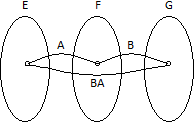
\includegraphics[width=0.4\linewidth]{compfunc.png}
		\end{center}
		\caption{Transformação linear composta BA}
		\label{fig:compfunc}
	\end{figure}
	
	Assim, podemos enunciar o seguinte teorema.
	\\ \newline \textbf{Teorema:} Sejam $A: E \longrightarrow F$ e $B: F \longrightarrow G$, $U = \{u_1, \dots, u_p\} \subset E$, $V = \{v_1, \dots, v_n\} \subset F$ e $W = \{w_1, \dots, w_m\} \subset G$ tal que $\mathbf{a} \in M(m\times p)$ é a matriz de $A$ nas bases $U, V$ e $\mathbf{b} \in M(m\times n)$ é a matriz de $B$ nas bases $V, W$, então a matriz de $BA: E\longrightarrow G$ nas bases $U, W$ é o produto $\mathbf{ba} \in M(m\times p)$ das matrizes $\mathbf{b}$ e $\mathbf{a}$. \cite{AlgebraLinearElon}
	\\
	
	Ou seja, se tivermos duas transformações lineares $A: E \longrightarrow F$ e $B: F \longrightarrow G$, podemos multiplicar suas representações matriciais $\mathbf{b}$ e $\mathbf{a}$ afim de obter o equivalente matricial da função composta $BA: E \longrightarrow G$. Este teorema é muito importante, podendo simplificar um algorítimo de $n$ operações lineares $\mathbf{a_i} \mid 1<i<n$ em apenas uma aplicação da forma $\mathbf{a_{r}x} = \mathbf{b}$, onde $\mathbf{a_{r}}$ é a matriz resultante de $\prod_{i=1}^{n}\mathbf{a}_i$.
	\\
	
	Assim concluímos o estudo sobre transformações lineares e suas representações como matrizes. Podemos aplicar estes conhecimentos em um caso específico de forte interesse neste documento, a matriz $B_i$.
	
	\subsubsection*{Sobre a Matriz $B_i$}
	
	Ao trabalhar-se com dados vindos de experimentos de RMN, é fácil perceber que o sistema de coordenadas cartesianas não é a melhor forma para representar estes dados, pois não se sabe de antemão qual a posição de cada átomo estudado. Como alternativa, utiliza-se as coordenadas internas que, de forma muito semelhante ao sistema de coordenadas esféricas (normalmente visto em calculo no $\mathbb{R}^3$), faz uso de distâncias e ângulos para representar localizações. 
	
	Infelizmente temos um problema: as coordenadas internas não são muito agradáveis. Necessitam de constantes manipulações trigonométricas e possuem complicada interpretação geométrica, pois não dependem de um referencial fixo, ou seja, esse sistema de coordenadas não possui uma origem bem definida como em um plano cartesiano., diferentemente, nesse sistema a referencia se dá sempre partindo da localização atual. Pode-se dizer que a referência é sempre de dentro para fora. Talvez seja daí que venha o termo "coordenadas \textit{internas}", pois o referencial é o interior do ponto que se estuda. 
	
	 Dados os motivos citados, salvo a liberdade poética do autor, temos forte interesse de apresentar os resultados finais de um experimento de RMN em coordenadas cartesianas, ou seja, deve-se transformar coordenadas internas em cartesianas. Infelizmente isso não é uma tarefa fácil e depende muito da configuração espacial que compõe a molécula estudada. Pode-se dizer que o PGDM resume-se nesta transformação de coordenadas. Perceba a importância de se estudar a matriz que possui este papel, no caso, a $B_i$.
	 
	 Conforme apresentado na seção ~\ref{sec:bi}, a $B_i$ é a $i$-ésima matriz $4\times 4$ em um produtório de $i$ matrizes $4\times 4$ que, multiplicadas pelo vetor-coluna $(0,0,0,1)$ dão origem a realização do $i$-ésimo átomo $x_i$ da molécula estudada. Ou seja, 
	 $$ B_i \in M(4\times 4) \mid
	 B_{1}B_{2}\cdots B_{i}\begin{bmatrix}
	 0\\ 
	 0\\ 
	 0\\ 
	 1
	 \end{bmatrix}
	 = \begin{bmatrix}
	 x_{i1}\\ 
	 x_{i2}\\ 
	 x_{i3}\\ 
	 1
	 \end{bmatrix}
	 \:\forall\:  1< i < N,
	 $$
	 
	 onde $N$ é o número de átomos na molécula e o vetor-coluna $(x_{i1}, x_{i2}, x_{i3}, 1)$ é a realização do $i$-ésimo átomo da molécula, ou seja, tal vetor possui componentes que coincidem com as coordenadas do ponto onde está localizado tal átomo no $\mathbb{R}^3$.
	 
	 Como dito anteriormente, o produto de matrizes é uma forma eficiente de concatenar funções e sabemos também que cada matriz $B_i$, necessária para encontrar a $i$-ésima realização na molécula, pode ser vista como representação de uma transformação linear, ou seja, cada $B_i$ pode ser vista como a matriz que compõe todas as operações necessárias para passar da $x_{i-1}$ até a $x_i$ realização, logo
	 $$
	 (B_1 B_2 \cdots B_{i-1})
	 B_i
	 \begin{bmatrix}
	 0\\ 
	 0\\ 
	 0\\ 
	 1
	 \end{bmatrix}
	 = \begin{bmatrix}
	 x_{i1}\\ 
	 x_{i2}\\ 
	 x_{i3}\\ 
	 1
	 \end{bmatrix},
	 $$
	 onde $(B_1,B_2,\cdots,B_{i-1})$ é a matriz que representa todas as operações necessárias para chegar da $x_1$ até a $x_{i-1}$. Perceba que é como se caminhássemos pelas realizações das moléculas, onde sabemos exatamente para onde apontar (pelos ângulos $\theta$ e $\omega$) e exatamente o quanto caminhar (a distância $d$) para ir de uma molécula a outra.
	 
	 Logo, sabemos que a $B_i$ será composta por movimentos de translações e rotações, nos bastando descobrir quais para entende-la. Nos será útil definir estes dois tipos de transformações lineares, como segue:
	 \begin{itemize}
	 	\item \textbf{Translação:} Podemos resumir esta operação em um deslocamento.
	 	
	 	Seja o vetor $v = (a) \in \mathbb{R}$. Perceba que há uma relação biunívoca entre o espaço vetorial $\mathbb{R}$ e o conjunto $C$ de pontos na reta real, ou seja, $\forall \: v \in \mathbb{R} \:\exists! \: u \in C \mid v\equiv u$, logo, podemos movimentar o vetor $v$ de forma a fazer o ponto por ele representado na reta também se movimentar.
	 	
	 	Como faremos isso? É intuitivo imaginar que a solução seja uma função do tipo $f: \mathbb{R} \longrightarrow \mathbb{R} \mid f(x) = (x + 1)$, ou seja, uma função que leva um ponto $x$ para uma unidade mais longe da origem. Infelizmente isso não se trata de uma movimentação, mas sim de um teleporte. Veja, o ponto mudou de lugar instantaneamente! Isso fere a linearidade:
	 	$$f(x+a) = x+a+1 \neq f(x)+f(a) = x+a+2$$ 
	 	
	 	Isso se deve pois quando algo é deslocado ele possui uma velocidade $\frac{\partial}{\partial t}$ associada, ou seja, precisamos deslocá-lo em relação a alguma dimensão específica do espaço vetorial (no caso $t$), logo, precisamos incrementar uma dimensão ao universo de nossa reta para encontrar a transformação linear que desloca um elemento $v$ por ela.
	 	
	 	Fazemos então 
	 	$$f: \mathbb{R}^2 \longrightarrow \mathbb{R} \mid f(x,t) = x+t,$$
	 	ou seja, agora o ponto $x$ ficará uma unidade mais distante da origem assim que a dimensão $t$ também o ficar. Perceba que agora $x$ movimenta-se a medida que $t$ movimenta, sem saltos, logo, respeitando a linearidade
	 	$$f((x,t)+(a,a)) = f(x+a, t+a) = x+t+a+a = f(x,t)+f(a,a).$$
	 	
	 	Como toda transformação linear pode ser escrita como uma matriz, segue que se
	 	$$
	 	f(x,t) = 
	 	\begin{bmatrix}
	 	1 & 1\\
	 	\end{bmatrix}
	 	\begin{bmatrix}
	 	x\\
	 	t
	 	\end{bmatrix}
	 	=
	 	\begin{bmatrix}
	 	x+t
	 	\end{bmatrix}
	 	= x+t
	 	$$
	 	então $\begin{bmatrix} 1 & 1 \end{bmatrix}$ é a matriz que representa tal transformação, nossa translação.
	 	
	 	%preciso falar sobre aquela algebra que almenta uma dimensão na matriz.. esqueci o nome dela :/ Não posso falar nada sem saber o nome :/
	 	
	 	\item \textbf{Rotação:} Quando se quer rotacionar um objeto, sem alterar o formato dele, normalmente recorremos a matrizes de rotação.
	 	
	 	Tentemos definir um operador que rotacione um vetor em um ângulo $\theta$  em torno da origem \cite{AlgebraLinearElon}, ou seja, precisamos de uma transformação linear $R: \mathbb{R}^2 \longrightarrow \mathbb{R}^2$ que, dado um vetor $v = (x,y) \in \mathbb{R}^2$, seja $Rv = (x', y')$. Como
	 	$$
	 	Rv = 
	 	\begin{bmatrix}
	 	a & b\\
	 	c & d
	 	\end{bmatrix}
	 	\begin{bmatrix}
	 	x\\
	 	y
	 	\end{bmatrix}
	 	=
	 	\begin{bmatrix}
	 	x'\\
	 	y'
	 	\end{bmatrix},
	 	$$
		então $x' = ax + by$ e $y' = cx + dy$. 
		
		Perceba que nosso objetivo é encontrar $a,b,c$ e $d$.
		Sabemos que se $B_{\mathbb{R}^2} = \{(1,0),(0,1)\}$ é a base canônica do $\mathbb{R}^2$, então $R(1,0) = (a,c)$ e $R(0,1) = (b,d)$. Por construção, se rotacionarmos os versores $(1,0)$ e $(0,1)$ em um ângulo $\theta$, conforme Figura ~\ref{fig:rota}, seguindo as definições de senos e cossenos, obtemos que $R(1,0) = (cos(\theta), sen(\theta))$ e $R(0,1) = (-sen(\theta), cos(\theta))$.
		
		\begin{figure}[H]
			\begin{center}
				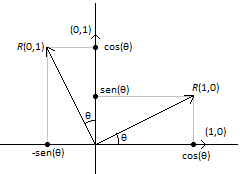
\includegraphics[width=0.5\linewidth]{rota.png}
			\end{center}
			\caption{Transformação linear composta BA}
			\label{fig:rota}
		\end{figure}
	 
	 	Logo, $x' = x cos(\theta) - y sen(\theta)$ e $y' = x sen(\theta) + y cos(\theta)$. Nossa matriz de rotação em torno da origem fica:
	 	$$
	 	\begin{bmatrix}
	 		a & b\\
	 		c & d
	 	\end{bmatrix}
	 	=
	 	\begin{bmatrix}
	 	cos(\theta) & -sen(\theta)\\
	 	sen(\theta) & cos(\theta)
	 	\end{bmatrix}.
	 	$$
	 	
	 	Podemos enxergar esta rotação como uma projeção de uma transformação no espaço tridimensional $\mathbb{R}^3$, onde a rotação acontece ao redor do eixo $z$ (que sai do papel), mantendo o eixo fixo. Para tentarmos ampliar esta matriz para a terceira dimensão, basta que nós entendamos que as componentes da transformação devem ser tais que não modifiquem componentes no eixo z, logo:
	 	$$
	 	\begin{bmatrix}
	 	cos(\theta) & -sen(\theta)\\
	 	sen(\theta) & cos(\theta)
	 	\end{bmatrix}
	 	\begin{bmatrix}
	 	x\\
	 	y
	 	\end{bmatrix}
	 	=
	 	\begin{bmatrix}
	 	x'\\
	 	y'
	 	\end{bmatrix}
	 	\longrightarrow
	 	\begin{bmatrix}
	 	cos(\theta) & -sen(\theta)&0\\
	 	sen(\theta) & cos(\theta)&0\\
	 	0 & 0 & 1
	 	\end{bmatrix}
	 	\begin{bmatrix}
	 	x\\
	 	y\\
	 	z
	 	\end{bmatrix}
	 	=
	 	\begin{bmatrix}
	 	x'\\
	 	y'\\
	 	z'
	 	\end{bmatrix},
	 	$$
	 	
	 	onde $z' = z$.
	 	
	 	A mesma lógica pode ser aplicada para deduzir as rotações em torno dos demais eixos, onde todas são enunciadas a seguir.
	 	
	 	$$
	 	R_x(\theta)\cdot(x,y,z) =
	 	\begin{bmatrix}
	 	1 & 0 & 0\\
	 	0&cos(\theta) & -sen(\theta)\\
	 	0&sen(\theta) & cos(\theta)
	 	\end{bmatrix}
	 	\begin{bmatrix}
	 	x\\
	 	y\\
	 	z
	 	\end{bmatrix}
	 	=
	 	\begin{bmatrix}
	 	x'\\
	 	y'\\
	 	z'
	 	\end{bmatrix},
	 	$$
	 	
	 	$$
	 	R_y(\theta)\cdot(x,y,z) =
	 	\begin{bmatrix}
	 	cos(\theta)&0 & -sen(\theta)\\
	 	0 & 1 & 0\\
	 	sen(\theta) & 0&cos(\theta)
	 	\end{bmatrix}
	 	\begin{bmatrix}
	 	x\\
	 	y\\
	 	z
	 	\end{bmatrix}
	 	=
	 	\begin{bmatrix}
	 	x'\\
	 	y'\\
	 	z'
	 	\end{bmatrix}.
	 	$$
	 	
	 	$$
	 	R_z(\theta)\cdot(x,y,z) =
	 	\begin{bmatrix}
	 	cos(\theta) & -sen(\theta)&0\\
	 	sen(\theta) & cos(\theta)&0\\
	 	0 & 0 & 1
	 	\end{bmatrix}
	 	\begin{bmatrix}
	 	x\\
	 	y\\
	 	z
	 	\end{bmatrix}
	 	=
	 	\begin{bmatrix}
	 	x'\\
	 	y'\\
	 	z'
	 	\end{bmatrix},
	 	$$
	 \end{itemize}	
 
 \newpage
 	Agora que possuímos tais definições, podemos voltar a analisar nossa $B_i$. Então, anunciando-a, sendo $i=4, \dots, N$:
 	$$
 	B_i\:=\:{
 		\begin{bmatrix}
 		-\cos(\theta_{i-2,i}) & -\mbox{sen}(\theta_{i-2,i}) & 0 & -d_{i-1,i}\cos(\theta_{i-2,i})\\ 
 		\mbox{sen}(\theta_{i-2,i})\cos(\omega_{i-3,i}) & -\cos(\theta_{i-2,i})\cos(\omega_{i-3,i})
 		& -\mbox{sen}(\omega_{i-3,i}) & d_{i-1,i}\mbox{sen}(\theta_{i-2,i})\cos(\omega_{i-3,i})\\ 
 		\mbox{sen}(\theta_{i-2,i})\mbox{sen}(\omega_{i-3,i}) & -\cos(\theta_{i-2,i})\mbox{sen}(\omega_{i-3,i}) & \cos(\omega_{i-3,i}) & d_{i-1,i}\mbox{sen}(\theta_{i-2,i})\mbox{sen}(\omega_{i-3,i})\\ 
 		0 & 0 & 0 & 1
 		\end{bmatrix},}
 	$$
 	
 	Pode-se deduzir, decompondo esta matriz em tentativas de composições com as matrizes de translação e rotações descritas, que esta matriz trata-se de 
 	$$
 	B_i=R_{x}(w_{i-3,i}).R_{x}(\pi).R_{z}(\theta_{i-2,i}).R_{y}(\pi).T_{x}(d_{i-1,i}),
 	$$
 	
 	onde, perceba, as operações são compostas da direita para a esquerda, ou seja, primeiro há uma translação e depois um conjunto de quatro rotações. Dentre essas, duas são de um angulo fixo $\pi$, isto se deve ao fato de que, como estamos caminhando de um átomo a outro, toda vez que chegamos em um novo átomo deve-se primeiro olhar para trás (para o átomo anterior) e só então definir aonde está a próxima direção à se percorrer, pois os ângulos assim são definidos (vide Figura ~\ref{fig:angulos}).
 	
 	\newpage
 	\phantomsection
 	\addcontentsline{toc}{section}{Apêndice C - Vinte Aminoácidos Naturais}
 	\section*{Apêndice C} 
 	
 	É comum dividirmos os aminoácidos proteicos em cinco classes, como segue.
 	\subsubsection*{Grupos R apolares, alifáticos}
 	\begin{figure}[H]
 		\begin{center}
 			\begin{minipage}{0.24\linewidth}
 				\centering   
 				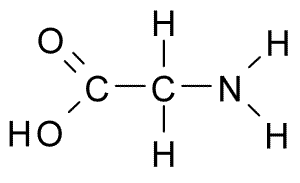
\includegraphics[width=0.95\linewidth]{glycine.png}	
 				\caption{Glicina}
 				\label{fig:glycine}
 			\end{minipage}
 			\begin{minipage}{0.24\linewidth}
 				\centering   
 				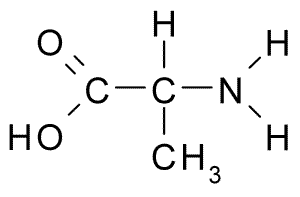
\includegraphics[width=0.9\linewidth]{alanine.png}
 				\caption{Alanina}
 				\label{fig:alanine}
 			\end{minipage}
 			\begin{minipage}{0.24\linewidth}
 				\centering   
 				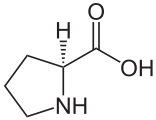
\includegraphics[width=0.8\linewidth]{proline.png}
 				\caption{Prolina}
 				\label{fig:proline}
 			\end{minipage}
	 		\begin{minipage}{0.24\linewidth}
		 		\centering   
		 		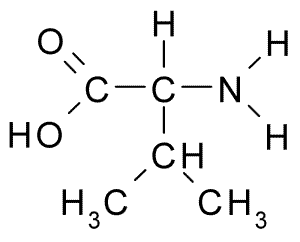
\includegraphics[width=0.8\linewidth]{valine.png}
		 		\caption{Valina}
		 		\label{fig:valine}
		 	\end{minipage}
 		\end{center}
 	\end{figure}
 	\vspace{-1cm}
 	\begin{figure}[H]
 		\begin{center}
 			\begin{minipage}{0.3\linewidth}
 				\centering   
 				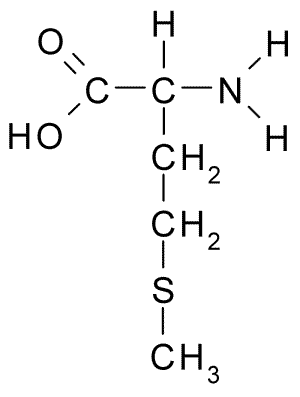
\includegraphics[width=0.63\linewidth]{methionine.png}	
 				\caption{Metionina}
 				\label{fig:methionine}
 			\end{minipage}
 			\begin{minipage}{0.3\linewidth}
 				\centering   
 				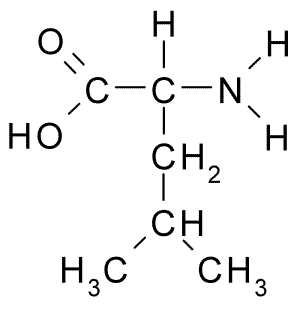
\includegraphics[width=0.8\linewidth]{leucine.png}
 				\caption{Leucina}
 				\label{fig:leucine}
 			\end{minipage}
 			\begin{minipage}{0.3\linewidth}
 				\centering   
 				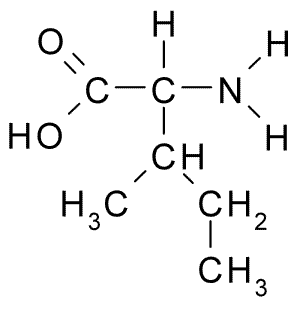
\includegraphics[width=0.8\linewidth]{isoleucine.png}
 				\caption{Isoleucina}
 				\label{fig:isoleucine}
 			\end{minipage}
 		\end{center}
 	\end{figure}
 
 	\subsubsection*{Grupos R polares, não carregados}	
 	
 	\begin{figure}[H]
 	\begin{center}
 		\begin{minipage}{0.3\linewidth}
 			\centering   
 			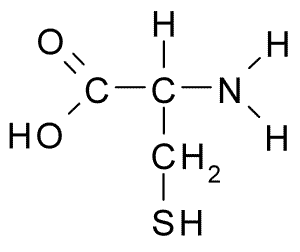
\includegraphics[width=0.8\linewidth]{cysteine.png}	
 			\caption{Cisteína}
 			\label{fig:cysteine}
 		\end{minipage}
 		\begin{minipage}{0.3\linewidth}
 			\centering   
 			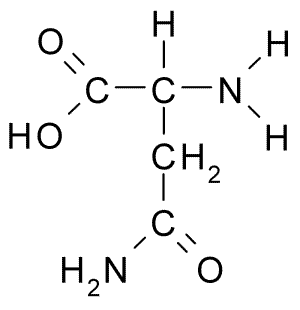
\includegraphics[width=0.65\linewidth]{asparagine.png}
 			\caption{Asparagina}
 			\label{fig:asparagine}
 		\end{minipage}
 		\begin{minipage}{0.3\linewidth}
 			\centering   
 			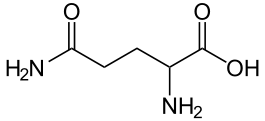
\includegraphics[width=1\linewidth]{glutamine.png}
 			\caption{Glutamina}
 			\label{fig:glutamine}
 		\end{minipage}
 	\end{center}
 	\end{figure}
	 \vspace{-1cm}
	\begin{figure}[H]
		\begin{center}
			\begin{minipage}{0.45\linewidth}
				\centering   
				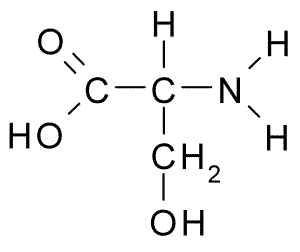
\includegraphics[width=0.5\linewidth]{serine.png}	
				\caption{Serina}
				\label{fig:serine}
			\end{minipage}
			\begin{minipage}{0.45\linewidth}
				\centering   
				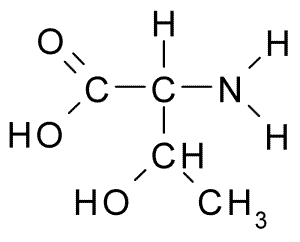
\includegraphics[width=0.5\linewidth]{threonine.png}
				\caption{Treonina}
				\label{fig:threonine}
			\end{minipage}
		\end{center}
	\end{figure}
 	
	\subsubsection*{Grupos R aromáticos}
	\begin{figure}[H]
		\begin{center}
			\begin{minipage}{0.3\linewidth}
				\centering   
				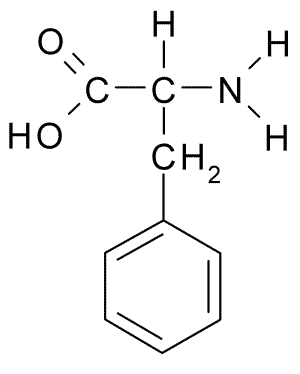
\includegraphics[width=0.7\linewidth]{phenylalanine.png}	
				\caption{Fenilalanina}
				\label{fig:phenylalanine}
			\end{minipage}
			\begin{minipage}{0.3\linewidth}
				\centering   
				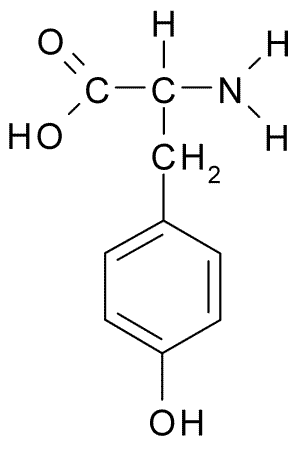
\includegraphics[width=0.59\linewidth]{tyrosine.png}
				\caption{Tirosina}
				\label{fig:tyrosine}
			\end{minipage}
			\begin{minipage}{0.3\linewidth}
				\centering   
				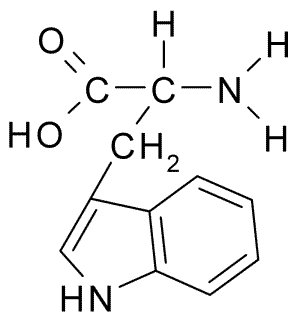
\includegraphics[width=0.7\linewidth]{tryptophan.png}
				\caption{Triptofano}
				\label{fig:tryptophan}
			\end{minipage}
		\end{center}
	\end{figure}
 	
 	\subsubsection*{Grupos R carregados positivamente}
 	\begin{figure}[H]
	 	\begin{center}
	 		\begin{minipage}{0.3\linewidth}
	 			\centering   
	 			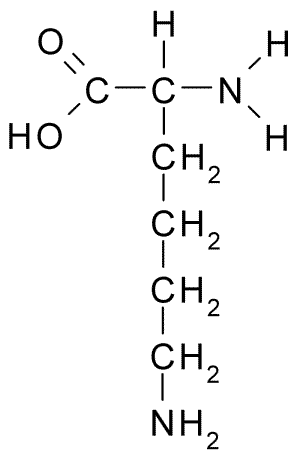
\includegraphics[width=0.7\linewidth]{lysine.png}	
	 			\caption{Lisina}
	 			\label{fig:lysine}
	 		\end{minipage}
	 		\begin{minipage}{0.3\linewidth}
	 			\centering   
	 			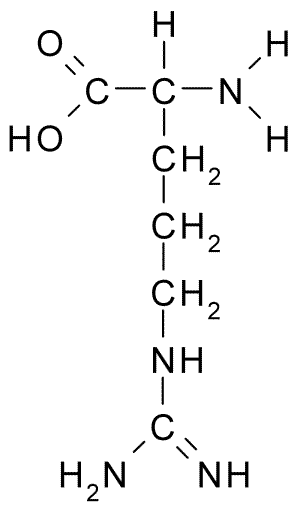
\includegraphics[width=0.59\linewidth]{arginine.png}
	 			\caption{Arginina}
	 			\label{fig:arginine}
	 		\end{minipage}
	 		\begin{minipage}{0.3\linewidth}
	 			\centering   
	 			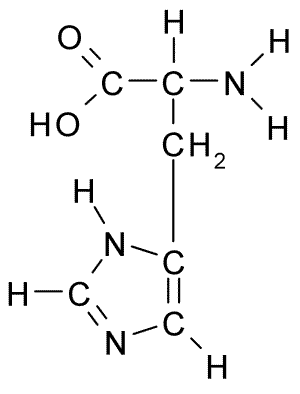
\includegraphics[width=0.7\linewidth]{histidine.png}
	 			\caption{Histidina}
	 			\label{fig:histidine}
	 		\end{minipage}
	 	\end{center}
	 \end{figure}
 
 	\subsubsection*{Grupos R carregados negativamente}
 	
 	\begin{figure}[H]
 		\begin{center}
 			\begin{minipage}{0.45\linewidth}
 				\centering   
 				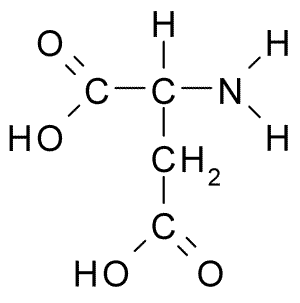
\includegraphics[width=0.5\linewidth]{asparticacid.png}	
 				\caption{Aspartato}
 				\label{fig:asparticacid}
 			\end{minipage}
 			\begin{minipage}{0.45\linewidth}
 				\centering   
 				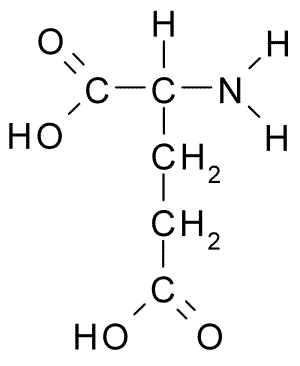
\includegraphics[width=0.45\linewidth]{glutamicacid.png}
 				\caption{Glutamato}
 				\label{fig:glutamicacid}
 			\end{minipage}
 		\end{center}
 	\end{figure}
 
 	
\end{document}